% В этом файле следует писать текст работы, разбивая его на
% разделы (section), подразделы (section) и, если нужно,
% главы (chapter).

% Предварительно следует указать необходимую информацию
% в файле SETUP.tex

%% В этот файл не предполагается вносить изменения

% В этом файле следует указать информацию о себе
% и выполняемой работе.

\documentclass [fontsize=14pt, paper=a4, pagesize, DIV=calc]%
{scrartcl}
% ВНИМАНИЕ! Для использования глав поменять
% scrartcl на scrreprt

% Здесь ничего не менять
\usepackage [T2A] {fontenc}   % Кириллица в PDF файле
\usepackage [utf8] {inputenc} % Кодировка текста: utf-8
\usepackage [russian] {babel} % Переносы, лигатуры

%%%%%%%%%%%%%%%%%%%%%%%%%%%%%%%%%%%%%%%%%%%%%%%%%%%%%%%%%%%%%%%%%%%%%%%%
% Создание макроса управления элементами, специфичными
% для вида работы (курс., бак., маг.)
% Здесь ничего не менять:
\usepackage{ifthen}
\newcounter{worktype}
\newcommand{\typeOfWork}[1]
{
	\setcounter{worktype}{#1}
}

% ВНИМАНИЕ!
% Укажите тип работы: 0 - курсовая, 1 - бак., 2 - маг.,
% 3 - бакалаврская с главами.
\typeOfWork{1}
% Считается, что курсовая и бак. бьются на разделы (section) и
% подразделы (subsection), а маг. — на главы (chapter), разделы и
%  подразделы. Если хочется,
% чтобы бак. была с главами (например, если она большая),
% надо выбрать опцию 3.

% Если при выборе 2 или 3 вы забудете поменять класс
% документа на scrreprt (см. выше, в самом начале),
% то получите ошибку:
% ./aux/appearance.tex:52: Package scrbase Error: unknown option ` chapterprefix=

%%%%%%%%%%%%%%%%%%%%%%%%%%%%%%%%%%%%%%%%%%%%%%%%%%%%%%%%%%%%%%%%%%%%%%%%
% Информация об авторе и работе для титульной страницы

\usepackage {titling}

% Имя автора в именительном падеже (для маг.)
\newcommand {\me}{%
И.\,И.~Иванов%
}

% Имя автора в родительном падеже (для курсовой и бак.)
\newcommand {\byme}{%
О.\,Е.~Филиппской%
}

% Любимый научный руководитель
\newcommand{\supervisor}%
{асс. каф. ИВЭ А.\,М. Пеленицын}

% идентифицируем пол (только для курсовой и бак.)
\newcommand{\bystudent}{
Студентки % Для курсовой: с большой буквы
}

% Год публикации
\date{2016}

% Название работы
\title{Генерация экземпляров классов типов\\на на основе экземпляров производных классов\\в языке Haskell}

% Кафедра
%
\newboolean{needchair}
\setboolean{needchair}{true} % на ФИИТ не пишется (false), на ПМИ есть (true)

\newcommand {\thechair} {%
Кафедра информатики и вычислительного эксперимента%
}

\newcommand {\direction} {%
Направление подготовки\\
Прикладная математика и информатика%
}% Прикладная математика и информатика

%%%%%%%%%%%%%%%%%%%%%%%%%%%%%%%%%%%%%%%%%%%%%%%%%%%%%%%%%%%%%%%%%%%%%%%%
% Другие настраиваемые элементы текста

% Листинги с исходным кодом программ: укажите язык программирования
\usepackage{listings}
\lstset{
    language=[ISO]C++,%  Язык указать здесь
    basicstyle=\small\ttfamily,
    breaklines=true,%
    deletekeywords={Monad,Functor,return,liftM,ap},
    morekeywords={where, instance, data, class, of},
    showstringspaces=false%
    inputencoding=utf8x%
    literate={\{}{\textcolor{black}{\{}}1
             {\}}{\textcolor{black}{\}}}1
             {[}{\textcolor{black}{[}}1     
             {]}{\textcolor{black}{]}}1
}
% полный список языков, поддерживаемых данным пакетом, есть,
% например, здесь (стр. 13):
% ftp://ftp.tex.ac.uk/tex-archive/macros/latex/contrib/listings/listings.pdf

% Нумерация списков: можно при необходимести
% изменять вид нумерации (например, добавлять правую скобку).
% По умолчанию буду списки вида:
% 1.
% 2.
% Изменять вид нумерации можно в начале нумерации:
% \begin{enumerate}[1)] (В квадратных скобках указан желаемый вид)
\usepackage[shortlabels]{enumitem}
                    \setlist[enumerate, 1]{1.}

% Гиперссылки: настройте внешний вид ссылок
\usepackage%
[pdftex,unicode,pdfborder={0 0 0},draft=false,%backref=page,
    hidelinks, % убрать, если хочется видеть ссылки: это
               % удобно в PDF файле, но не должно появиться на печати
    bookmarks=true,bookmarksnumbered=false,bookmarksopen=false]%
{hyperref}


\usepackage {amsmath}      % Больше математики
\usepackage {amssymb}
\usepackage {textcase}     % Преобразование к верхнему регистру
\usepackage {indentfirst}  % Красная строка первого абзаца в разделе

\usepackage {fancyvrb}     % Листинги: определяем своё окружение Verb
\DefineVerbatimEnvironment% с уменьшенным шрифтом
	{Verb}{Verbatim}
	{fontsize=\small}

% Вставка рисунков
\usepackage {graphicx}

% Общее оформление
% ----------------------------------------------------------------
% Настройка внешнего вида

%%% Шрифты

% если закомментировать всё — консервативная гарнитура Computer Modern
\usepackage{paratype} % профессиональные свободные шрифты
%\usepackage {droid}  % неплохие свободные шрифты от Google
%\usepackage{mathptmx}
%\usepackage {mmasym}
%\usepackage {psfonts}
%\usepackage{lmodern}
%var1: lh additions for bold concrete fonts
%\usepackage{lh-t2axccr}
%var2: the package below could be covered with fd-files
%\usepackage{lh-t2accr}
%\usepackage {pscyr}

% Геометрия текста

\usepackage{setspace}       % Межстрочный интервал
\onehalfspacing

\newlength\MyIndent
\setlength\MyIndent{1.25cm}
\setlength{\parindent}{\MyIndent} % Абзацный отступ
\frenchspacing            % Отключение лишних отступов после точек
\KOMAoptions{%
    DIV=calc,         % Пересчёт геометрии
    numbers=endperiod % точки после номеров разделов
}

                            % Консервативный вариант:
%\usepackage                % ручное задание геометрии
%[%                         % (не рекомендуется в проф. типографии)
%  margin = 2.5cm,
  %includefoot,
  %footskip = 1cm
%] %
%  {geometry}

%%% Заголовки

\ifthenelse{{\value{worktype} > 1}}{%
  \KOMAoptions{%
      headings=normal,   % размеры заголовков поменьше стандартных
      chapterprefix=true,% Печатать слово Глава
      appendixprefix=true% Печатать слово Приложение
  }
}{% Печатать слово Приложение даже если нет глав
  \newcommand*{\appendixmore}{%
%    \renewcommand*{\sectionformat}{%
%       \appendixname~\thesection\autodot\enskip}
    \renewcommand*{\sectionmarkformat}{%
      \appendixname~\thesection\autodot\enskip}
  }
}

% шрифт для оформления глав и названия содержания
\newcommand{\SuperFont}{\Large\sffamily\bfseries}

% Заголовок главы
\ifthenelse{\value{worktype} > 1}{%
\renewcommand{\SuperFont}{\Large\normalfont\sffamily}
\newcommand{\CentSuperFont}{\centering\SuperFont}
\usepackage{fncychap}
\ChNameVar{\SuperFont}
\ChNumVar{\CentSuperFont}
\ChTitleVar{\CentSuperFont}
\ChNameUpperCase
\ChTitleUpperCase
}

% Заголовок (под)раздела с абзацного отступа
\addtokomafont{sectioning}{\hspace{\MyIndent}}

\renewcommand*{\captionformat}{~---~}
\renewcommand*{\figureformat}{Рисунок~\thefigure}

% Плавающие листинги
\usepackage{float}
\floatstyle{ruled}
\floatname{ListingEnv}{Листинг}
\newfloat{ListingEnv}{htbp}{lol}[section]

% точка после номера листинга
\makeatletter
\renewcommand\floatc@ruled[2]{{\@fs@cfont #1.} #2\par}
\makeatother


%%% Оглавление
\usepackage{tocloft}

% шрифт и положение заголовка
\ifthenelse{\value{worktype} > 1}{%
\renewcommand{\cfttoctitlefont}{\hfil\SuperFont\MakeUppercase}
}{
\renewcommand{\cfttoctitlefont}{\hfil\SuperFont}
}

% слово Глава
\usepackage{calc}
\ifthenelse{\value{worktype} > 1}{%
\renewcommand{\cftchappresnum}{Глава }
\addtolength{\cftchapnumwidth}{\widthof{Глава }}
}

% Очищаем оформление названий старших элементов в оглавлении
\ifthenelse{\value{worktype} > 1}{%
\renewcommand{\cftchapfont}{}
\renewcommand{\cftchappagefont}{}
}{
\renewcommand{\cftsecfont}{}
\renewcommand{\cftsecpagefont}{}
}

% Точки после верхних элементов оглавления
\renewcommand{\cftsecdotsep}{\cftdotsep}
%\newcommand{\cftchapdotsep}{\cftdotsep}

\ifthenelse{\value{worktype} > 1}{%
    \renewcommand{\cftchapaftersnum}{.}
}{}
\renewcommand{\cftsecaftersnum}{.}
\renewcommand{\cftsubsecaftersnum}{.}
\renewcommand{\cftsubsubsecaftersnum}{.}

%%% Списки (enumitem)

\usepackage {enumitem}      % Списки с настройкой отступов
\setlist %
{ %
  leftmargin = \parindent, itemsep=.5ex, topsep=.4ex
} %

% По ГОСТу нумерация должны быть буквами: а, б...
%\makeatletter
%    \AddEnumerateCounter{\asbuk}{\@asbuk}{м)}
%\makeatother
%\renewcommand{\labelenumi}{\asbuk{enumi})}
%\renewcommand{\labelenumii}{\arabic{enumii})}

%%% Таблицы: выбрать более подходящие

\usepackage{booktabs} % считаются наиболее профессионально выполненными
%\usepackage{ltablex}
%\newcolumntype {L} {>{---}l}

%%% Библиография

\usepackage{csquotes}        % Оформление списка литературы
\usepackage[T1]{fontenc}
\usepackage[
  backend=biber,
  hyperref=auto,
  sorting=none, % сортировка в порядке встречаемости ссылок
  language=auto,
  citestyle=gost-numeric,
  bibstyle=gost-numeric
]{biblatex}
\addbibresource{biblio.bib} % Файл с лит.источниками

% Настройка величины отступа в списке
\ifthenelse{\value{worktype} < 2}{%
\defbibenvironment{bibliography}
  {\list
     {\printtext[labelnumberwidth]{%
    \printfield{prefixnumber}%
    \printfield{labelnumber}}}
     {\setlength{\labelwidth}{\labelnumberwidth}%
      \setlength{\leftmargin}{\labelwidth}%
      \setlength{\labelsep}{\dimexpr\MyIndent-\labelwidth\relax}% <----- default is \biblabelsep
      \addtolength{\leftmargin}{\labelsep}%
      \setlength{\itemsep}{\bibitemsep}%
      \setlength{\parsep}{\bibparsep}}%
      \renewcommand*{\makelabel}[1]{\hss##1}}
  {\endlist}
  {\item}
}{}

% ----------------------------------------------------------------
% Настройка переносов и разрывов страниц

\binoppenalty = 10000      % Запрет переносов строк в формулах
\relpenalty = 10000        %

\sloppy                    % Не выходить за границы бокса
%\tolerance = 400          % или более точно
\clubpenalty = 10000       % Запрет разрывов страниц после первой
\widowpenalty = 10000      % и перед предпоследней строкой абзаца

% ----------------------------


% Стили для окружений типа Определение, Теорема...
% Оформление теорем (ntheorem)

\usepackage [thmmarks, amsmath] {ntheorem}
\theorempreskipamount 0.6cm

\theoremstyle {plain} %
\theoremheaderfont {\normalfont \bfseries} %
\theorembodyfont {\slshape} %
\theoremsymbol {\ensuremath {_\Box}} %
\theoremseparator {:} %
\newtheorem {mystatement} {Утверждение} [section] %
\newtheorem {mylemma} {Лемма} [section] %
\newtheorem {mycorollary} {Следствие} [section] %

\theoremstyle {nonumberplain} %
\theoremseparator {.} %
\theoremsymbol {\ensuremath {_\diamondsuit}} %
\newtheorem {mydefinition} {Определение} %

\theoremstyle {plain} %
\theoremheaderfont {\normalfont \bfseries} 
\theorembodyfont {\normalfont} 
%\theoremsymbol {\ensuremath {_\Box}} %
\theoremseparator {.} %
\newtheorem {mytask} {Задача} [section]%
\renewcommand{\themytask}{\arabic{mytask}}%
\newtheorem {myremark} {Замечание} %

\theoremheaderfont {\scshape} %
\theorembodyfont {\upshape} %
\theoremstyle {nonumberplain} %
\theoremseparator {} %
\theoremsymbol {\rule {1ex} {1ex}} %
\newtheorem {myproof} {Доказательство} %

\theorembodyfont {\upshape} %
%\theoremindent 0.5cm
\theoremstyle {nonumberbreak} \theoremseparator {\\} %
\theoremsymbol {\ensuremath {\ast}} %
\newtheorem {myexample} {Пример} %
\newtheorem {myexamples} {Примеры} %

\theoremheaderfont {\itshape} %
\theorembodyfont {\upshape} %
\theoremstyle {nonumberplain} %
\theoremseparator {:} %
\theoremsymbol {\ensuremath {_\triangle}} %
\theoremstyle {nonumberbreak} %
\newtheorem {myremarks} {Замечания} %


% Титульный лист
% Макросы настройки титульной страницы
% В этот файл не предполагается вносить изменения

%\usepackage {showframe}

% Вертикальные отступы на титульной странице
\newcommand{\vgap}{\vspace{16pt}}

% Помещение города и даты в нижний колонтитул
\usepackage{scrlayer}
\DeclareNewLayer[
  foot,
  foreground,
  contents={%
    \raisebox{\dp\strutbox}[\layerheight][0pt]{%
      \parbox[b]{\layerwidth}{\centering Ростов-на-Дону\\ \thedate%
       \\\mbox{}
       }}%
  }
]{titlepage.foot.fg}
\DeclareNewPageStyleByLayers{titlepage}{titlepage.foot.fg}


\AtBeginDocument %
{ %
  %
  \begin{titlepage}
  %
    \thispagestyle{titlepage}

    {\centering
    %
    \MakeTextUppercase {МИНИСТЕРСТВО ОБРАЗОВАНИЯ И НАУКИ РФ}

    \vgap

    Федеральное государственное автономное образовательное\\
    учреждение высшего образования\\
    \MakeTextUppercase {Южный федеральный университет}

    \vgap

	Институт математики, механики и компьютерных наук
    имени~И.\,И.\,Воровича

    \vgap

    \direction

    \ifthenelse{\boolean{needchair}}{
    \vgap

    \thechair}{}

    \vspace* {\fill}

    \ifthenelse{\value{worktype} = 2}{%
    \me

    \vgap}{}

    {\usefont{T2A}{PTSansCaption-TLF}{m}{n}
    \MakeTextUppercase{\thetitle}}

    \ifthenelse{\value{worktype} = 2}{%
     \vgap

    Выпускная квалификационная работа\\
    на степень магистра}{}
    \ifthenelse{\value{worktype} = 0}{
     \vgap

    Курсовая работа
    }{}%
    \ifthenelse{\value{worktype} = 1 \OR \value{worktype} = 3}{
     \vgap

    Выпускная квалификационная работа\\
    на степень бакалавра
    }{}%

    \vspace {\fill}

    \begin{flushright}
    \ifthenelse{\value{worktype} = 0 \OR 
                \value{worktype} = 1 \OR
                \value{worktype} = 3}{
      \bystudent \ifthenelse{\value{worktype} = 0}{3}{4}\ курса\\
      \byme
    }{}

    \vgap

    Научный руководитель:\\
    \supervisor\\
    \ifthenelse{\value{worktype} = 2}{%
    Рецензент:\\
    ученая степень, ученое звание, должность
    И. О. Фамилия
    }{}
	\end{flushright}
    \ifthenelse{\value{worktype} = 0}{
    \vspace{\fill}
            \begin{flushleft}
              \begin{tabular}{cc}
                \underline{\hspace{4cm}}&\underline{\hspace{5cm}}\\
                {\small оценка (рейтинг)} & {\small  подпись руководителя}\\
              \end{tabular}
            \end{flushleft}
    }{}
  	\vspace {\fill}
  %Ростов-на-Дону

    %\thedate

  }\end{titlepage}
  %
  %
  \tableofcontents
  %
  \clearpage
} %



% Команды для использования в тексте работы


% макросы для начала введения и заключения
\newcommand{\Intro}{\addsec{Введение}}
\ifthenelse{\value{worktype} > 1}{%
    \renewcommand{\Intro}{\addchap{Введение}}%
}

\newcommand{\Conc}{\addsec{Заключение}}
\ifthenelse{\value{worktype} > 1}{%
    \renewcommand{\Conc}{\addchap{Заключение}}%
}

% Правильные значки для нестрогих неравенств и пустого множества
\renewcommand {\le} {\leqslant}
\renewcommand {\ge} {\geqslant}
\renewcommand {\emptyset} {\varnothing}

% N ажурное: натуральные числа
\newcommand {\N} {\ensuremath{\mathbb N}}

% значок С++ — используйте команду \cpp
\newcommand{\cpp}{%
C\nolinebreak\hspace{-.05em}%
\raisebox{.2ex}{+}\nolinebreak\hspace{-.10em}%
\raisebox{.2ex}{+}%
}

% Неразрывный дефис, который допускает перенос внутри слов,
% типа жёлто-синий: нужно писать жёлто"/синий.
\makeatletter
    \defineshorthand[russian]{"/}{\mbox{-}\bbl@allowhyphens}
\makeatother


\endinput

% Конец файла

\hyphenation{Monad Applicative Functor Control Data}
    \tikzstyle{every node}=[shape=rectangle, color=black, rounded corners,%
    text=black, anchor=west]
    \tikzstyle{selected}=[shape=rectangle, rounded corners,%
    top color=gray,%
    bottom color=gray, text=white]
    \tikzstyle{optional}=[dashed,fill=gray!50]
    \tikzset{
    	basic/.style  = {draw, text width=2cm, font=\sffamily, rectangle},
    	root/.style   = {basic, rounded corners=2pt, thin, align=center,
    		fill=white},
    	level 2/.style = {basic, rounded corners=6pt, thin,align=center, fill=white,
    		text width=8em}
    }

\begin{document}

\Intro
%\section*{Предварительные сведения}
В современном мире невозможно представить жизнь без компьютерных технологий. Они используются повсеместно в различных областях жизнедеятельности. В связи с этим бурно развивается сфера информационных технологий, появляется большое количество прикладного программного обеспечения, как открытого, так и проприетарного. Разработчики проприентарного ПО стремятся к расширению функционала, а также временной и ресурсовой оптимизации своих программ для того, чтобы их продукт смог выдержать конкуренцию на рынке аналогичного ПО. Не менее важным аспектом в разработке ПО является внедрение оригинальных (никем ранее не внедрённых) функциональных средств. Компания, в которой проводилась данная научно-исследовательская работа, занимается разработкой программного продукта, известного как Filter Forge. Это ПО для обработки и создания изображений и фильтров, аналогов которому на сегодняшний день не имеется.

С точки зрения внутренней структуры, Filter Forge~--- это доменно-специфичный язык (см. рис.~\ref{forge}), обладающий строгой статической типизацией, с ленивыми вычислениями и неизменяемыми состояниями.
\begin{figure}
	\centering
	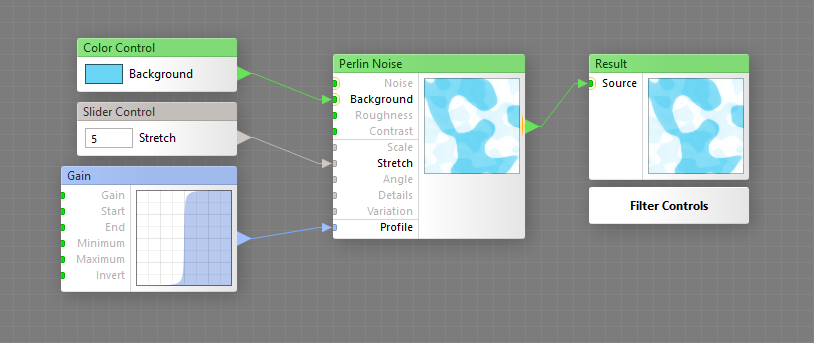
\includegraphics[width=\textwidth]{img/forge.png}
	\caption{Пример визуального синтаксиса Filter Forge}\label{forge}
\end{figure}
 Типами являются <<цвета>> компонентов. Система типов Filter Forge была спроектирована и разработана относительно давно (2002 - 2004 год). За это время требования к языку значительно изменились и старая реализация оказалась мало пригодной для дальнейшего ее развития. Поэтому компания начала поиск альтернатив среди современных языков программирования, обладающих свойствами, которые компания хотела бы видеть в реализации своего языка.

Один из самых популярных языков функционального программирования Haskell обладает всеми требуемыми свойствами~--- строгая статическая типизация, ленивые вычисления, неизменяемые состояния. Однако в дополнение к ним в Haskell также имеется параметрический полиморфизм, возможность создания произвольных типов данных, наконец, Haskell~--- тьюринг-полный язык. Однако синтаксис в Filter Forge визуальный (а не текстовый). Под влиянием этих данных автору и создателю Filter Forge приходит идея о функциональном языке программирования с визуальным синтаксисом, за основу  системы типов которого взята система типов языка Haskell. Типам и языкам программирования посвящена книга~\autocite{pierce}.

\section*{Цель работы}
В настоящее время в Filter Forge, Inc. ведётся разработка визуального функционального языка программирования. Работа над языков поделена на несколько частей:
 \begin{enumerate}[1)]
 	\item разработка IDE и одновременно с этим синтаксиса для него (поскольку синтаксис визуальный);
 	\item разработка системы типов;
 	\item разработка алгоритма вывода типов;
 	\item разработка кодогенератора.
 \end{enumerate} 

В рамках научно-исследовательской работы принималось участие в разработке алгоритма вывода типов. Целью работы была разработка алгоритма вывода типов в пределах одного компонента, разработка правил распространения информации о типах по компонентам, описывающим программу, а также проверка работоспособности разработанного и реализованного алгоритма в сравнении с языком-эталоном, в качестве которого был выбран язык Haskell.
\section*{Постановка задачи}
Поскольку разработка ведётся на языке C++, алгоритм вывода типов необходимо реализовать на C++. Таким образом, требуется:
\begin{enumerate}[1)]
	\item реализовать алгоритм вывода типов в пределах одного компонента с учётом уже существующей системы типов;
	\item реализовать алгоритм сортировки компонентов для дальнейшего распространения информации о типах по них;
	\item используя различные средства языка Haskell осуществить трансляцию программы на визуальном языке в программу на языке Haskell и проанализировать результаты работы.
\end{enumerate}
%\chapter{Предварительные сведения}

\chapter{Алгоритм вывода типов}\label{type_inf}
В этой главе мы рассмотрим алгоритм вывода типов, который был разработан для функционального языка программирования с визуальным синтаксисом. Алгоритм будет разделён на несколько элементарных случаев в зависимости от аргументов, которые будут ему поданы. В конце будет приведён алгоритм сортировки компонентов дерева программы для их последующего обновления. 
\section{Основные понятия}
Для начала введём основные термины, которые будут использоваться при описании алгоритма вывода типов.
\begin{description}
	\item[Компонент.] Компонентами являются встроенные функции. Примеры компонентов: см. рис. \ref{components}.
	\begin{figure}[h]
		\centering
		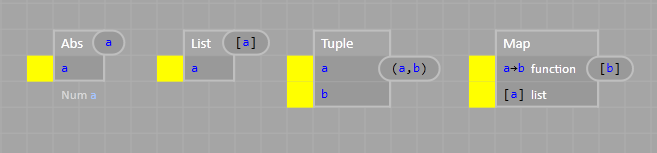
\includegraphics{img/components.PNG}
		\caption{Примеры компонентов}\label{components}	
	\end{figure}
	\item[Функция.] Если не указано иное, функцией будем называть определённую пользователем функцию. Пример функции: см. рис. \ref{customfun}.	
	\begin{figure}[h]
		\centering
		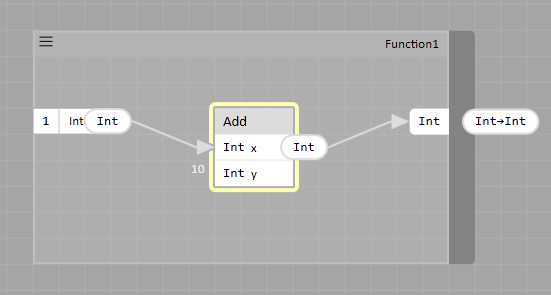
\includegraphics{img/custom_function.PNG}
		\caption{Пример функции, определённой пользователем}\label{customfun}	
	\end{figure}
	\item[Корневая функция, или корень.] Функция без параметров, определённая в глобальной области видимости, значение которой непосредственно требуется вычислить (см. рис.~\ref{corefun}). Чтобы её значение можно было вычислить, она должна быть неполиморфной, то есть её тип должен быть однозначно определён. Кроме того, у компонентов, из которых состоит её тело, не должно быть пустых входов: на входе должна быть либо связь, либо конкретное значение.
	\begin{figure}[h]
		\centering
		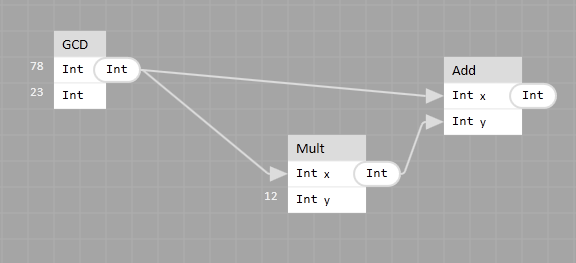
\includegraphics{img/core.PNG}
		\caption{Пример корневой функции}\label{corefun}	
	\end{figure}
	\item[Вызывающий компонент (caller).] Компонент, предназначающийся для использования определённой пользователем функции.
	\item[Вход (connection point).] Вход компонента соответствует одному аргументу функции, которой отвечает компонент. На вход можно подать значение (одно из возможных значений типа, который назначен данному входу) либо другой компонент. Компонент может не иметь входов, если это: 
	\begin{enumerate}[1)]
		\item аргумент определяемой пользователем функции;
		\item вызывающий компонент (caller) пользовательской функции без аргументов.
	\end{enumerate} 
	Пустой вход обозначается жёлтым цветом.
	\item[Связь (connection).] Если один компонент подан другому на вход в качестве аргумента, то будем говорить, что между этими компонентами существует связь. Также между компонентами может существовать неявная связь, если явной связи (в виде стрелочки) нет, то, тем не менее, изменения в одном компоненте приводят к изменениям в другом. Такая связь существует между функцией и её вызывающим компонентом.
	\item[Унификация (unify).] Две переменные типа унифицированы, если их ограничения не противоречат друг другу. Если две переменные унифицированы, то это значит, что они взаимозаменяемы.
	\item[Ограничение (constraint).] Будем говорить, что переменная имеет ограничение, если выполняется одно или более из условий:
		\begin{enumerate}[1)]
			\item переменная унифицирована с одной или более другими переменными (\textit{ограничение унификации});
			\item переменная принадлежит одному или нескольким классам типов (\textit{ограничение классов типов});
			\item переменная имеет конкретный тип, например, \lstinline!Int!, \lstinline!Bool!, \lstinline!Char! и т.д. (\textit{ограничение конкретного типа}).
		\end{enumerate}  
	Ограничения могут противоречить друг другу. Например, если на переменную, принадлежащую классу типов \textit{Num} по валидной на данный момент связи придёт тип \textit{Char}. В таком случае связь, по которой пришли противоречивые ограничения и компонент, в который они пришли, объявляются мёртвыми (dead). В IDE это отображается красным цветом (см. рис. \ref{dead}).	
	\begin{figure}[h]
		\centering
		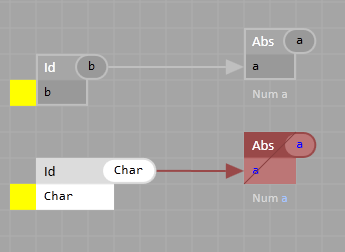
\includegraphics{img/dead.PNG}
		\caption{Пример мёртвого компонента}\label{dead}
	\end{figure}
	
	\item[Контекст.] Контекстом будем называть набор всех ограничений на все переменные отдельно взятого компонента. Каждый компонент имеет свой отдельный контекст.
	\item[Идентификатор входа.] Для того, чтобы различать, какая переменная контекста какому входу соответствует введём идентификаторы входов. Идентификатора входа однозначно идентифицирует номер входа конкретного компонента; входы компонентов нумеруются с нуля.
	\item[Собственные переменные.] Собственными переменными контекста будем называть те переменные, которые находились в контексте с момента создания компонента.
	\item[Импортированые переменные.] Импортированными переменными будем называть те переменные, которые попали в текущий контекст по связям из контекстов других компонентов.
	\item[Параметр.] При описании алгоритма вывода типов переменную типа для удобства будем называть параметром.
	\item[Конкретный тип (value type).] К конкретным типам отнесём типы \lstinline|Int|, \lstinline|Float|, \lstinline|Char|, \lstinline|Bool|, а также кортежи \lstinline|(a1, a2, ...)|, списки \lstinline|[a]|, и тому подобное. Таким образом, внутри конкретного типа могут иметься другие типы.
	%\item[Инферер (inferer).] description
	\item[Псевдоним (alias).] Новое имя, которое может получить параметр в процессе вывода типов.
\end{description}


\section{Общие правила}
Пусть имеется дерево программы, в котором уже произошёл вывод типов. Предположим, что какой-то компонент инициировал новый вывод типов, т.\,е. произошло одно из следующих событий:
\begin{enumerate}[1)]
	\item была убрана или добавлена какая-либо связь со входом этого компонента;
	\item по уже существующей связи пришли новые данные (ограничения), т.\,е. изменение произошло в более левом компоненте, и до текущего дошло обновление;
	\item на какой-либо из переменных компонента был явно указан новый тип;
	\item если данный компонент вызывающий, то изменился тип аргументов или результата функции, которую он вызывает.
\end{enumerate}
Допустим также, что этот вывод затронул тип результата компонента. Тогда дальше вывод типов будет происходить во всех компонентах, связь к которым идёт от текущего. Этот процесс назовём \textit{пропагацией} (от англ. \textit{propagation}~--- распространение). Если же в процессе вывода типов результат компонента не изменился, тогда пропагация останавливается. Результат компонента мог не измениться по следующим причинам:
\begin{enumerate}[1)]
	\item результат имеет конкретный тип, не зависящий от входов;
	\item произошедшие изменения не добавили никаких принципиально новых ограничений на переменную типа результата.
\end{enumerate}
Также пропагация останавливается в том случае, если обновление дошло до компонента, не имеющего исходящих связей (ни явных, ни неявных).

Пусть в контексте какого-либо компонента есть несколько переменных. Пусть $a_1, a_2, \ldots, a_n$~--- \textit{собственные} переменные текущего контекста, $b_1, b_2, \ldots, b_m$~--- \textit{импортированные} переменные. И пусть какие либо переменные $a_{i_1}, a_{i_2}, \ldots, a_{i_k}$ и $b_{j_1}, b_{j_2}, \ldots, b_{j_l}$ унифицированы с переменной результата. Нужно принять решение, какие из этих переменных будут скопированы в другой контекст, один или несколько входов которого связаны с результатом текущего. Тогда копироваться будут все переменные, кроме собственных переменных контекста, т.\,е. $b_{j_1}, b_{j_2}, \ldots, b_{j_l}$.


\section{Алгоритм вывода типов в простейшем случае}
Теперь рассмотрим алгоритм вывода типов в отдельно взятом компоненте. В таком случае возможно 3 варианта, в которых мы будем действовать по-разному. Рассмотрим пример простейшей связи двух компонентов, рис. \ref{connection}. Контекст правого компонента будем считать текущим. Контекст левого компонента назовём \textit{внешним}.

\begin{figure}[h]
	\centering
	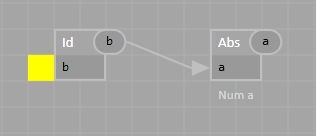
\includegraphics{img/connection.PNG}
	\caption{Пример простейшей связи двух компонентов}\label{connection}
\end{figure}

\textit{На вход} алгоритму подаётся два типа. Один из внешнего контекста, который находится на его результате. Второй тип из текущего контекста, который находится на входе, в который пришёл тип из внешнего компонента.

\textit{Результатом} алгоритма будет сообщение о том, произошло ли текущее выведение успешно или же оно завершилось с ошибкой. Кроме того, если один из аргументов был параметром, и выведение типов завершилось успешно, то этот параметр получит новое ограничение.

\subsection{Параметр против параметра}\label{algo}
Пусть в текущем контексте имеется параметр, на котором уже есть ограничения. Обозначим этот параметр $a_n$, где $n$~--- идентификатор входа этого параметра. Пусть через вход компонента, соответствующего идентификатору входа $n$, попадает другой параметр, со своим набором ограничений, обозначим его $b_n$. Нам нужно принять решение, можно ли унифицировать $a_n$ и $b_n$. Для этого ограничения на этих параметрах проверяются на непротиворечивость по следующему алгоритму.
\begin{enumerate}
	\item Собрать все ограничения (классов типов и конкретного типа), которые имеются на $a_n$. Для этого нужно также собрать все известные ограничения на переменных, с которыми $a_n$ унифицирован.
	\item Скопировать $b_n$ со всеми его ограничениями в текущий контекст. Также собрать все указанные ограничения, которые на нём имеются.
	\item Проверить, что классы типов, которым принадлежат $a_n$ и $b_n$ не противоречат друг другу (если они имеются). Для этого множество классов типов $b_n$ должно быть подмножеством классов типов $a_n$. Если это не так, то переходим на последний пункт.
	\item Проверить, что конкретные типы, если таковые имеются, друг другу не противоречат, см. подглаву \ref{valueVSvalue}. Если это не так, переходим на последний пункт.
	\item Если противоречий не выявлено, тогда алгоритм завершается успешно(см. замечание~\ref{rem_fur_prop}), и указанные переменные унифицируются. Таким образом, на $a_n$ и на $b_n$ появляются новые ограничения унификации.
	\item Если в процессе вывода типа были найдены противоречивые ограничения, то алгоритм завершается с ошибкой (см. замечание~\ref{rem_imp_prop}). Связь и текущий компонент помечаются мёртвыми.	
\end{enumerate}

\myremark{
	Алгоритм завершается успешно, если в процессе вывода типов не было выявлено противоречий. Это означает, что возможна дальнейшая пропагация типов.
}\label{rem_fur_prop}
\myremark{
	Если на текущем шаге алгоритм вывода типов завершился с ошибкой, то дальнейшая пропагация невозможна.
}\label{rem_imp_prop}

\subsection{Конкретный тип против параметра}
Пусть нужно провести вывод параметра против конкретного типа. Обозначим параметр как $a_n$, где $n$~--- идентификатор входа, конкретный тип как $Val_1(x_1, x_2, \ldots, x_m)$. Тогда алгоритм будет заключаться в следующем.
\begin{enumerate}
	\item Если $a_n$ не принадлежит текущему контексту (например, зашёл в текущий компонент по связи), тогда копируем его в текущий контекст.
	\item Собираем все известные ограничения параметра $a_n$.
	\item Проверяем, что классы типов, которым принадлежит параметр, не противоречат классам типов, экземпляром которых является $Val_1(x_1, x_2, \ldots, x_m)$. Это означает, что множество классов типов, которым принадлежит $a_n$, должно быть подмножеством классов типов, экземпляром которых является $Val_1(x_1, x_2, \ldots, x_m)$. Если это не так, тогда алгоритм типов прерывается, связь и компонент объявляются мёртвыми.
	\item Для каждого $x_i, i = 1 .. m$ необходимо выполнить следующие действия. Если $x_i$~--- это параметр:
		\begin{enumerate}[1)]
			\item если $x_i$ уже есть в текущем контексте, провести вывод типов параметр против параметра; если он завершился с ошибкой, тогда вывод типов останавливается;
			\item если $x_i$ нет в текущем контексте, тогда скопировать его в текущий контекст со всеми ограничениями. Пометить этот параметр (см. замечание \ref{rem_rec_types}).
		\end{enumerate}	
	Допустим теперь, что $x_i$~--- конкретный тип. Обозначим его $Val_3(z_1, z_2, \ldots, z_l)$:
		\begin{enumerate}[1)]
			\item если $l = 0$, т.\,е $Val_3$ имеет род $*$, тогда ничего делать не нужно;
			\item если же $Val_3$ имеет род $* \rightarrow \ldots \rightarrow *$, тогда выполнить для него пункт 6.
		\end{enumerate}
	\item Если на параметре имеется ограничение в виде конкретного типа $Val_2(y_1, y_2, \ldots, y_k)$, то см. главу \ref{valueVSvalue}. Если вывод $Val_1(x_1, x_2, \ldots, x_m)$ на $Val_2(y_1, y_2, \ldots, y_k)$ завершился с ошибкой, то связь и компонент объявляются мёртвыми и вывод типов прерывается.
	\item Если на предыдущих шагах не возникло ошибки, тогда на параметр $a_n$ добавляется ограничение конкретного типа $Val_1(x_1, x_2, \ldots, x_m)$.
	\item Если ни на каком из предыдущих шагов не возникло ошибки, тогда алгоритм завершается успешно.
\end{enumerate}

\myremark{
	Поясним, для чего нужно помечать параметры. Дело в том, что при выводе типов для рекурсивной функции есть опасность получить бесконечный тип. Например, если на параметр $a_n$ добавить ограничение $[a_n]$, то мы получим бесконечное множество раз вложенный список. Допустим, параметр $a_n$ помечен. Тогда при попытке пометить его второй раз, уже в качестве внутреннего параметра списка, станет ясно, что мы имеем дело с бесконечным типом. В таком случае вывод типов прерывается, связь и текущим компонент объявляются мёртвыми.
}\label{rem_rec_types}

\subsection{Конкретный тип против конкретного типа}\label{valueVSvalue}
Пусть в текущем контексте имеется конкретный тип, который обозначим $Val_1 (x_1, x_2, \ldots, x_k)$, где $x_1, x_2, \ldots, x_k$~--- внутренние параметры или внутренние конкретные типы $Val_1$. Их может и не быть, если тип имеет род $*$ (англ. \textit{kind}). Пусть теперь через вход, соответствующий идентификатору входа $n$, поступает конкретный тип $Val_2 (y_1, y_2, \ldots, y_l)$. Нам необходимо убедиться, что эти типы друг другу не противоречат.
\begin{enumerate}
	\item Убедимся, что $Val_1$ и $Val_2$ являются конструкторами одного и того же типа. Если это так, и, кроме того, они имеют род $*$, тогда алгоритм завершается успешно. Если же типы имеют род $* \rightarrow \ldots \rightarrow *$, тогда переходим на шаг 2.
	\item Проверим, что $k == l$, т.\,е. что количества внутренних типов совпадают. Например, если и $Val_1$, и $Val_2$ представляют собой конструкторы кортежей $Tuple$, то нужно проверить, что это кортежи из одинакового количества элементов. Если это не так, тогда алгоритм завершается, а связь и текущий компонент помечаются мёртвыми.
	\item Для каждой пары типов $(x_i, y_i), i = 1 .. k$ применить соответствующий ей простейший алгоритм вывода типов.	Но перед этим каждый из этих параметром необходимо \textit{пометить} (см. замечание \ref{rem_rec_types}).
\end{enumerate}

\section{Алгоритм определения порядка обновления компонентов в дереве}\label{alg_order}
Рассмотрим синтаксическое дерево программы языка с точки зрения теории графов. Здесь \textit{вершины}~--- это компоненты, \textit{дуги}~--- это связи между компонентами. Вспомним, что связь может быть:
	\begin{enumerate}[1)]
		\item явной, т.\,е. стрелкой между результатом одного компонента и входом другого;
		\item неявной, такая связь имеется между функцией и её вызывающим компонентом.
	\end{enumerate}
Поскольку функция может быть рекурсивной, на графе могут присутствовать циклы. Кроме того, могут также быть определены функции, которые нигде не вызываются. Это значит, что подграф этой функции может не иметь исходящих связей. Предположим также, что ни один компонентов из корня не участвует в определении функции, то есть её подграф не имеет и входящих связей. Таким образом, граф программы может быть несвязным.

Итак, пусть какой-либо компонент в дереве инициировал обновление. Прежде чем начать вывод типов, определим, какие компоненты могут быть затронуты в результате этого изменения. Нам нужно получить упорядоченный список компонентов, чтобы затем согласно этому списку проводить пропагацию. Получим его с помощью следующего алгоритма.

\textit{Входные данные:} компонент, инициировавший изменение, синтаксическое дерево программы.

\textit{Результат работы:} список компонентов, которые необходимо обновить, в том порядке, в котором их следует обновлять.

\begin{enumerate}
	\item Для начала нужно получить список всех компонентов, достижимых из компонента-инициатора. Компонент является достижимым, если до него существует путь по дугам нашего графа. Получим такой список с помощью известного алгоритма \textit{поиска в глубину} [ссылка на алгоритм].
	\item Теперь у нас есть подграф всех компонентов, достижимых из инициатора. Обозначим этот подграф $G(V, E)$, где $V$~--- это множество вершин, $E$~--- множество дуг. Построим \textit{конденсацию} этого подграфа. Пусть $C(V', E')$~-- конденсация, $V'$~--- её вершины, $E'$~--- её дуги. Вершинами являются \textit{компоненты сильной связности} графа (см. замечание \ref{rem_ssc}). Дуга от $V_i \in V'$ к $V_j \in V'$ проводится, если найдутся такие вершины $u, v \in V$, что $u \in V_i, v \in V_j$, и существует дуга $(u, v)$.
	\item Строим \textit{топологическую сортировку} конденсации $C(V', E')$. Поскольку компоненты, не принадлежащие циклам, образуют отдельные КСС (см. замечание \ref{rem_ssc}), то порядок обновления этих компонентов будет таким же, как порядок соответствующих КСС в топологической сортировке.
	\item Внутри КСС, содержащих циклы, порядок обновления компонентов определяется следующим образом. Допустим, инициатор находится вне цикла. Пусть пропагация обновлений дошла до одного из компонентов цикла, по отношению к циклу он является инициатором. Тогда строим топологическую сортировку для подграфа текущей КСС без нового компонента-инициатора.
\end{enumerate}

\myremark{
	В нашем случае может быть два типа компонент сильной связности. Первый тип~--- КСС, состоящая из единственного компонента. Второй тип~--- цикличный подграф рекурсивной (возможно взаимнорекурсивной) функции(й). Таким образом, в КСС может быть либо ровно один компонент, либо не менее трёх (в случае простейшей рекурсивной функции: результат этой функции, сама функция, её вызывающий компонент внутри её тела).
}\label{rem_ssc}
%\subsection{Проверка типов на независимость}
%В процессе вывода типов рекурсивной 

%\chapter{Проблемы и их решения}

\chapter{Детали реализации}
В этой главе будет приведена реализация алгоритма вывода типов, описанного в главе~\ref{type_inf}. Сначала будет рассказано о классах, которые были определены и использованы. Здесь же выясним, какие средства языка C++ помогли более эффективно работать с объектами. Затем перейдём к реализации основной функции вывода типов~--- \lstinline!infer_type!. Наконец, будет определена функция сортировки компонентов.  
\section{Определения классов}
Поскольку все операции проводятся над типами, был определён специальный интерфейс \lstinline!Type!. Методы этого интерфейса:
\begin{enumerate}[1)]
	\item \lstinline!void enum_parameters(unique_parameter_ids_set& parameters) const!: проходит по все внутренним типам, находит среди них параметры и упорядочивает их;
	\item \lstinline!TypeClass::Class get_type_class(void) const!: возвращает множество классов типов, которым принадлежит тип;
	\item  \lstinline!size_t get_inner_types_count(void) const!: возвращает количество внутренних типов;
	\item \lstinline!const TypeRef& get_inner_type(const size_t index) const!: возвращает один внутренний тип по его номеру.
\end{enumerate}

Для работы с \lstinline!Type! определим класс \lstinline!TypeRef!:
\begin{figure}[H]
	\begin{lstlisting}
class TypeRef : public std::shared_ptr<const Type>
	\end{lstlisting}
\end{figure}
Ниже мы поясним, для чего здесь используется разделённый указатель (анлг. \textit{shared pointer}).

Рассмотрим классы, реализующие интерфейс \lstinline!Type!. Первый из них~--- \lstinline!ValueType!. Описывает конкретный тип. Члены этого класса:
	\begin{enumerate}[1)]
		\item \lstinline!m_type_info!, представляет собой \lstinline!const!-ссылку на \lstinline!TypeInfo!, содержит такую информацию о типе, как его имя, идентификатор (см. ниже), ограничение на количество внутренних типов;
		\item \lstinline!m_inner_types!, список внутренних типов, представляет собой \lstinline!vector<TypeRef>!.
	\end{enumerate}
Второй класс~--- это \lstinline!TypeParameter!, описывает переменную типа (параметр). Здесь члены класса:
\begin{enumerate}[1)]
	\item \lstinline!m_type_inferer!, указатель на контекст, в котором находится этот параметр;
	\item \lstinline!m_id!, уникальный (в пределах глобальной области видимости) идентификатор параметра (см. замечание~\ref{rem_par_id});
\end{enumerate}
\myremark{
	Уникальный идентификатор параметра складывается из буквы, которую он получил при создании, и уникального номера контекста, в котором он был создан. Контексты нумеруются в порядке создания компонентов, не зависимо от имени самого компонента.
}\label{rem_par_id}

\begin{figure}[H]
	\centering
	\begin{tikzpicture}[
	level 1/.style={sibling distance=60mm},
	edge from parent/.style={<-,draw},
	>=latex]
		\node[root] {Type}
			child {node[level 2] (c1) {ValueType}}
			child {node[level 2] (c2) {TypeParameter}};
	\end{tikzpicture}
	\caption{Иерархия классов}\label{hier}
\end{figure}

Определим также пару вспомогательных типов:
\begin{figure}[H]
	\begin{lstlisting} 
typedef std::shared_ptr<const ValueType> ValueTypeRef;
typedef std::shared_ptr<const TypeParameter> TypeParameterRef;
	\end{lstlisting}
\end{figure}
Эти типы позволяют хранить разделённый указатель не на базовый абстрактный интерфейс, а на непосредственно дочерний класс.
Использование разделённых указателей позволяет эффективно использовать один и тот же объект в нескольких местах. При этом, за счёт встроенного счетчика ссылок, удаление объекта будет произведено только в момент удаления последней ссылки на этот объект. Копирование такого объекта приводит только лишь к увеличению счётчика ссылок объекта, эта операция не является затратной по времени и памяти.

Также класс \lstinline!std::shared_ptr<>! позволяет хранить указатель на один и тот же объект по ссылке на разные типы. Поясним эту идею на следующем примере:
\begin{figure}[H]
	\begin{lstlisting}
TypeRef type = TypeRef::create(TypeId::Int);
ValueTypeRef int_type = type.evaluate();
	\end{lstlisting}
\end{figure}
Оба объекта (и \lstinline!type!, и \lstinline!int_type!) указывают на один и тот же объект, только объект \lstinline!type! при этом содержит указатель типа \lstinline!const Type*!, а \lstinline!int_type! содержит указатель типа \lstinline!const ValueType*!. Счётчик ссылок для каждого объекта равен двум.

Это свойство объектов класса \lstinline!shared_ptr<>! активно используется во время проведения операции вывода типов, которую мы рассмотрим в следующей подглаве.

\section{Определение функции infer\_types}
%\subsection{Параметр против параметра}
%\subsection{Конкретный тип против параметра}
%\subsection{Конкретный тип против конкретного типа}

Рассмотрим реализацию фрагмента алгоритма вывода типов, описанную в главе 1.3.
Согласно этому алгоритму нам необходимо рассмотреть три случая:
\begin{enumerate}[1)]
	\item параметр против параметра;
	\item параметр против конкретного типа;
	\item конкретный тип против конкретного типа.
\end{enumerate}
Случай <<конкретный тип против параметра>> легко сводится к случаю <<параметр против конкретного типа>> перестановкой местами типов, участвующих в выводе.

Полная реализация алгоритма приводиться не будет в связи с громоздкостью.

Итак, функция \lstinline!infer_types! имеет следующий прототип:
\begin{figure}[H]
	\begin{lstlisting}
InferenceResult infer_types(const TypeRef& source_type, const TypeRef& target_type, InferenceContext& context);
	\end{lstlisting}
\end{figure}
Она получает два типа, которые нужно вывести (по указателю на базовый класс), а также структуру \lstinline!context! (она имеет тип \lstinline!InferenceContext! и содержит различную информацию о подстановках параметров и прочих настройках текущей сессии вывода типов).
Возвращает функция результат вывода типов (либо <<OK>> (успешное завершение операции, см. гл.~\ref{algo}, замечание~\ref{rem_fur_prop}), либо структуру, описывающую причину останова операции).

Как уже было сказано ранее, наш алгоритм требует информации о фактических типах аргументов (т.е. является аргумент параметром или конкретным типом). Для получения этой информации воспользуемся шаблоном проектирования Посетитель (англ. \textit{Visitor}).

В классе \lstinline!TypeRef! опишем следующий метод:
\begin{figure}[H]
	\begin{lstlisting}
void visit(ITypeVisitor& visitor) const;
	\end{lstlisting}
\end{figure}
Здесь \lstinline!ITypeVisitor!~--- это интерфейс, имеющий следующее описание(см. листинг~\ref{ivis}):
\begin{ListingEnv}[H]
	\begin{lstlisting}
class ITypeVisitor
{
public:
  virtual void visit(const ValueTypeRef& value) = 0;
  virtual void visit(const TypeParameterRef& parameter) = 0;
}
	\end{lstlisting}
	\caption{Интерфейс ITypeVisitor}\label{ivis}
\end{ListingEnv}

Объект класса \lstinline!TypeRef! определяет, ссылка на какой из двух типов хранится внутри него, после чего преобразует себя к \lstinline!shared_ptr<>!-типу, разделённому указателю на нужный дочерний тип, и вызывает метод \lstinline!visit! объекта \lstinline!ITypeVisitor!, переданного ему параметром. Таким образом, для конкретных типов всегда будет вызываться функция принимающая объект типа \lstinline!ValueTypeRef!, а для параметров будет всегда вызываться другая функция (с аргументом типа \lstinline!TypeParameterRef!).

В реализации метода \lstinline!infer_types()! встречается служебная структура \lstinline!UnifiedData! (см. листинг~\ref{uni_data}). Эта структура описывает все ограничения, наложенные на какой-либо параметр в текущем контексте. Её поля:
\begin{itemize}
	\item уникальный идентификатор: имя запрашиваемого параметра;
	\item список параметров, с которыми унифицирован запрашиваемый параметр;
	\item объединение множеств классов типов, которым принадлежат все унифицированные параметры;
	\item список ограничений конкретного типа (с идентификаторами входа).
\end{itemize}

\begin{ListingEnv}[H]
	\begin{lstlisting}
struct UnifiedData
{
  UniqueParameterId original_id;
  std::set<UniqueParameterId> unified_names;
  TypeClass::Class type_class;
  values_with_origins_list values;
}
	\end{lstlisting}
	\caption{Определение структуры UnifiedData}\label{uni_data}
\end{ListingEnv}


Теперь перейдем непосредственно к рассмотрению реализации метода \lstinline!infer_types()! (см. листинг~\ref{infer_proto}). Разобьём реализацию этой функции на несколько частей, каждую из которых снабдим описанием.
\begin{ListingEnv}[H]
	\begin{lstlisting}
InferenceResult TypeInferer::infer_types(const TypeRef& source_type, const TypeRef& target_type, InferenceContext& context)
	\end{lstlisting}
	\caption{Прототип функции infer\_types}\label{infer_proto}
\end{ListingEnv}
	Описываем лямбда-функцию, которая будет вызываться для параметр-типов (см. листинг~\ref{lambda_par}).
	Функция копирует параметр (вызов метода \lstinline!copy_parameter_data()!) в текущий контекст (если необходимо) и собирает все ограничения этой переменной в структуру \lstinline!unified_data!.
	Возвращаемое значение лямбда-функции~--- результат вывода типов, он может содержать сообщение об ошибке, если какая-либо из вложенных операций завершится с ошибкой.
\begin{ListingEnv}[h]
	\begin{lstlisting}
{	
CollectDataVisitor::parameter_functor_type on_parameter = [&](UnifiedData& unified_data, const TypeParameterRef& parameter, const origins_type& origins)
{
	const ParameterId& id = parameter->get_id();
	UniqueParameterId uid = id.unique_id;
	if (id.current_context != &m_parent)
	{
		ParameterData* result;
		RET_ON_COPY_FAIL(result, copy_parameter_data(id, context, origins))
		uid = result->id;
	}
	unified_data = collect_unified_data(uid);
	return InferenceResult();
};
	\end{lstlisting}
	\caption{Лямбда-функция для параметр-типов}\label{lambda_par}
\end{ListingEnv}

	Описываем лямбда-функцию, которая будет вызываться для конкретных типов (см. листинг~\ref{lambda_val}).
	Функция копирует в текущий контекст все параметры, которые встречаются среди внутренних типов текущего конкретного типа, и создает структуру \lstinline!unified_data!, которая содержит только один этот конкретный тип.
	Также возвращает результат вывода типов (может быть ошибкой в случае ошибочного завершения какой-либо вложенной операции.)
	
\begin{ListingEnv}[h]
	\begin{lstlisting}
	
CollectDataVisitor::value_functor_type on_value = [&](UnifiedData& unified_data, const ValueTypeRef& value, const origins_type& origins)
{
	RET_ON_FAIL(deep_copy_parameters(value, nullptr, context, origins))
	unified_data = UnifiedData(value, origins);
	return InferenceResult();
};
	\end{lstlisting}
	\caption{Лямбда-функция для конкретных типов}\label{lambda_val}
\end{ListingEnv}
		Запуск операции (см. листинг~\ref{call_op}). Здесь через ранее описанный вызов метода visit() определяется фактический тип объектов \lstinline!source_type! и \lstinline!target_type!, после чего для них вызываются соответствующие им лямбда-функции, описанные ранее.
	
\begin{ListingEnv}[h]
	\begin{lstlisting}
UnifiedData source_data;
RET_ON_FAIL(CollectDataVisitor::collect(source_type, source_data, context.source_origins, on_value, on_parameter))
UnifiedData target_data;
RET_ON_FAIL(CollectDataVisitor::collect(target_type, target_data, context.target_origins, on_value, on_parameter))
	\end{lstlisting}
	\caption{Запуск операции}\label{call_op}
\end{ListingEnv}
		Помечаем параметры, если они есть (см. листинг~\ref{mark_guard}). Если при попытке пометить параметр оказывается, что пометка на ней уже есть, то операция вывода типов завершается с ошибкой (попытка создания саморекурсивного типа).
	
\begin{ListingEnv}[h]
	\begin{lstlisting}
ProcessGuard guard(m_parent);
for (const auto& current : source_data.unified_names)
	RET_ON_FAIL(guard.process_parameter(find(current)))
for (const auto& current : target_data.unified_names)
	RET_ON_FAIL(guard.process_parameter(find(current)))
	\end{lstlisting}
	\caption{Расстановка пометок на параметрах}\label{mark_guard}
\end{ListingEnv}
		Проводим проверку ограничений (см. листинг~\ref{check}). %Реализация функции \lstinline!check_unification()! является реализацией алгоритма описанного в главе 1.3.
		В случае, если проверка унификации завершается с ошибкой, выполнение функции \lstinline!infer_types! прерывается досрочно с пробросом кода ошибки в вызывающую функцию.
\begin{ListingEnv}[H]
	\begin{lstlisting}	
RET_ON_FAIL(check_unification(source_data, target_data, context))
	\end{lstlisting}
	\caption{Проверка ограничений}\label{check}
\end{ListingEnv}

К этому моменту мы проверили, что типы, переданные функции в качестве параметров не содержат противоречивых ограничений. Поэтому теперь функция должна добавить в текущий контекст новые ограничения, которые зависят от того, какие типы выводились:
\begin{itemize}
	\item параметр против параметра: унифицируем два параметра (см. листинг~\ref{unify});
	\item конкретный тип против параметра: добавить конкретный тип к параметру (см. листинг~\ref{value});
	\item параметр против конкретного типа: добавить конкретный тип к параметру (см. листинг~\ref{value2}).
\end{itemize}

\begin{ListingEnv}[h]
	\begin{lstlisting}
const bool empty_source = source_data.unified_names.empty();
const bool empty_target = target_data.unified_names.empty();
if (empty_source == empty_target)
  {
    if (!empty_source)
      return add_unify_constraint(find(source_data.original_id),   find(target_data.original_id), context, context.target_origins);
    }
	\end{lstlisting}
	\caption{Унификация двух параметров}\label{unify}
\end{ListingEnv}

\begin{ListingEnv}[h]
	\begin{lstlisting}
    else
    {
      if (empty_source)
      {
       const InferenceContext::SwapOrigins swap_origins(context);
       const TypeRef& max = TypeRef::max_polymorph_type(source_data.values);
       return add_value_constraint(find(target_data.original_id), max.as_value(), context);
      }
	\end{lstlisting}
	\caption{Добавление ограничения типа}\label{value}
\end{ListingEnv}

\begin{ListingEnv}[h]
	\begin{lstlisting}
      else
      {
        const TypeRef& max = TypeRef::max_polymorph_type(target_data.values);
        return add_value_constraint(find(source_data.original_id), max.as_value(), context);
      }
    }
	\end{lstlisting}
	\caption{Добавление ограничения типа}\label{value2}
\end{ListingEnv}

Случай конкретный тип против конкретного типа сам по себе новых ограничений не добавляет, однако ограничения могут добавиться от вывода его внутренних типов. Это произойдет на рекурсивном вызове функции \lstinline!infer_types()!, вызов которой находится в теле функции \lstinline!check_unification()!.

В конце возвращаем код <<OK>> об успешном завершении текущей операции вывода типов (см. листинг~\ref{OK}).
    
\begin{ListingEnv}[h]
	\begin{lstlisting}
  return InferenceResult();
}
	\end{lstlisting}
	\caption{Возврат сообщения об успехе}\label{OK}
\end{ListingEnv}

\section{Реализация алгоритма определения порядка обновления компонентов}
Здесь будет приведена реализация алгоритма, описанного в главе~\ref{alg_order}.
\subsection{Вспомогательные структуры данных}
В этой подглаве расскажем об особенностях вспомогательных структур данных, которые нам понадобятся.

Для реализации алгоритма обхода в глубину нам необходимо будет расставлять метки на вершинах графа. Между разными запусками обхода в глубину эти метки нужно будет восстановить к исходным (т.\,е. меткам, которые присутствовали на вершинах графа до начала текущего обхода). Организуем программу так, чтобы эти метки восстанавливались автоматически. Для этого реализуем класс \lstinline!VisitedStateGuard! (см. листинг~\ref{VSGclass}). Членом этого класса будет ассоциативный список, ключом которого является указатель на компонент, а значением~--- состояние отметки о посещении этого компонента до момента совершения обхода. Метод этого класса: \lstinline!void invert(const Component::VisitedState state1, const Component::VisitedState state2)!, у всех компонентов, имеющих состояние посещения \lstinline!state1!, заменяет его на состояние \lstinline!state2!, и наоборот (позднее мы поясним, для чего это нужно);

Кроме того, важным в реализации данного класса явлется реализация его \textit{деструктора} (см. листинг~\ref{VGSdestr}). Деструктор для объекта вызывается в конце области видимости этого объекта. Область видимости можно изменить самостоятельно, ограничив её скобками. Таким образом, обозначив нужную нам область видимости для объекта класса \lstinline!VisitedStateGuard!, мы регулируем, в какой момент вызовется деструктор. Таким образом, метки с вершин графа будут сняты автоматически (как нам и хотелось).

\begin{ListingEnv}
	\begin{lstlisting}
class VisitedStateGuard
{
public:
	VisitedStateGuard(const ComponentManager& component_manager, Component::VisitedState visited_state);
	~VisitedStateGuard();
	
	void invert(const Component::VisitedState state1, const Component::VisitedState state2);

private:
	typedef std::map<const Component*, Component::VisitedState> visited_state_type;
	
	visited_state_type m_state;
};		
	\end{lstlisting}
	\caption{Класс VisitedStateGuard}\label{VSGclass}
\end{ListingEnv}

\begin{ListingEnv}
	\begin{lstlisting}
VisitedStateGuard::~VisitedStateGuard()
{
    for (auto item : m_state)
        item.first->set_visited_state(item.second);
}
	\end{lstlisting}
	\caption{Деструктор класса VisitedGuardState}\label{VGSdestr}
\end{ListingEnv}

\subsection{Реализация функции sort\_components}
Переходим к рассмотрению реализации функции \lstinline! sort_components! (см. листинг~\ref{sort_proto}), в которой и будет происходить сортировка. Эта функция принимает 2 аргумента:
\begin{enumerate}[1)]
	\item \lstinline!manager!: ссылка на объект класса \lstinline!ComponentManager!; всё, что здесь нужно о нём знать, это то, что в нём содержится информация обо всех компонентах, задействованных в программе;
	\item \lstinline!initiator!: ссылка на компонент, инициирующий обновление. 
\end{enumerate}

\begin{ListingEnv}[h]
	\begin{lstlisting}
std::list<Component*> sort_components(const ComponentManager& manager, Component& initiator)		
	\end{lstlisting}
	\caption{Прототип функции sort\_components}\label{sort_proto}
\end{ListingEnv}

Теперь подготовимся к обходу (см. листинг~\ref{prepare}). Создадим граф \lstinline!scc_graph!. Это объект класса \lstinline!Graph!, этот класс является представлением ориентированного графа и предоставляет стандартные методы для работы с ним (включая топологическую сортировку). Ограничим количество вершин в нём количеством компонентов, имеющихся в программе. Это граф будущей конденсации. Затем объявим ассоциативный список \lstinline!component_to_vertex_map!, ключом в котором является указатель на компонент, а значением -- соответствующий этому компоненту номер его компоненты связности, т.\,е. номер вершины в графе-конденсации. Также объявим список указателей на компоненты \lstinline!out_order!. Сюда, согласно пункту 1 алгоритма из главы~\ref{alg_order}, поместим все компоненты, достижимые из компонента-инициатора.
\begin{ListingEnv}[h]
	\begin{lstlisting}
{	
typedef Graph<sorted_components_type> graph_type;

graph_type scc_graph(manager.get_components_count());
std::map<const Component*, size_t> component_to_vertex_map;
sorted_components_type out_order;
	\end{lstlisting}
	\caption{Подготовка к обходу}\label{prepare}
\end{ListingEnv}

Итак, следующий блок кода (см. листинг~\ref{dfs_scc}) помещён в фигурные скобки для того, чтобы ограничить область видимости для переменной объекта  \lstinline!visited_guard!. Создаём этот объект, запоминая, какие метки были на компонентах до вызова функции \lstinline!sort_components!. Затем совершаем обход в глубину, после которого в списке \lstinline!out_order! окажутся компоненты, достижимые из инициатора (код функции \lstinline!straight_dfs! приводить не будем, поскольку он не представляет интереса). 

\tikzstyle{vertex}=[circle,fill=black!25,minimum size=20pt,inner sep=1pt]
\tikzstyle{selected vertex} = [vertex, fill=red!24]
\tikzstyle{edge} = [draw, thick, ->]

Теперь нам нужно провести так называемый обратный обход в глубину. Он должен затронуть те вершины, которые мы уже прошли (сейчас имеют пометку "посещена"), и не должен пройти по вершинам, соответствующим компонентам, которые обновляться в текущей сессии вывода типов не будут (т.е. имеют пометку "не посещена"). Тогда сделаем следующее: пусть прямой обход в глубину произведён, и граф имеет следующее состояние (см. рис.~\ref{graph_ex}): знаком <<$+$>> помечены посещённые алгоритмом вершины, знаком <<$-$>> отмечены непосещённые вершины, красным цветом изображён инициатор. 
\begin{figure}[h]
	\centering	
	\begin{tikzpicture}[scale=1.8, auto, swap]
	\node[vertex](1) at (0, 0) {$-$};
	\node[vertex](2) at (1, 0) {$-$};
	\node[selected vertex](3) at (2, 0) {$+$};
	\node[vertex](4) at (3, 0) {$+$};
	\node[vertex](5) at (4, 0) {$+$};
	\node[vertex](6) at (3.5, 1) {$+$};
	\foreach \source/\dest in {1/2, 2/3, 3/4, 4/5, 5/6, 6/4}
	\path[edge](\source) -- (\dest);
	\end{tikzpicture}
	\caption{Пример графа обхода компонентов}\label{graph_ex}
\end{figure}
Тогда вызовем метод \lstinline!invert! для объекта \lstinline!visited_guard! с параметрами \lstinline!UNVISITED!, \lstinline!VISITED!, тогда все посещённые вершины станут непосещёнными и наоборот, и граф приобретёт следующий вид (см. рис.~\ref{graph_after_invert}). 
\begin{figure}[h]
	\centering	
	\begin{tikzpicture}[scale=1.8, auto, swap]
	\node[vertex](1) at (0, 0) {$+$};
	\node[vertex](2) at (1, 0) {$+$};
	\node[selected vertex](3) at (2, 0) {$-$};
	\node[vertex](4) at (3, 0) {$-$};
	\node[vertex](5) at (4, 0) {$-$};
	\node[vertex](6) at (3.5, 1) {$-$};
	\foreach \source/\dest in {1/2, 2/3, 3/4, 4/5, 5/6, 6/4}
	\path[edge](\source) -- (\dest);
	\end{tikzpicture}
	\caption{Графа обхода компонентов после замены меток}\label{graph_after_invert}
\end{figure}
Теперь обратный алгоритм обхода в глубину пройдёт только по интересующим нас вершинам. Далее организуем цикл по всем найденным достижимым компонентам. В этом цикле будут найдены компоненты сильной связности при помощи алгоритма \textit{Косараю-Шарира} (реализацию алгоритма в более общем виде можно найти здесь:~\autocite{emax_topo}). Таким образом, в графе \lstinline!scc_graph! появились вершины. По завершении этого программного блока объект класса \lstinline!visited_guard! будет разрушен, за счёт чего метки с него будут сняты.


\begin{ListingEnv}
	\begin{lstlisting}
{
    VisitedStateGuard visited_guard(manager, Component::VisitedState::UNVISITED);
    straight_dfs(initiator, out_order);

    visited_guard.invert(Component::VisitedState::UNVISITED, Component::VisitedState::VISITED);
    for (auto location = out_order.rbegin(); location != out_order.rend(); ++location)
    {
        if ((*location)->get_visited_state() == Component::VisitedState::UNVISITED)
        {
           sorted_components_type scc;
           reverse_dfs(**location, scc);
           auto vertex = scc_graph.ensure_vertex(scc);
           
           for (auto component : scc)
              component_to_vertex_map.insert(std::make_pair(component, vertex.index));
        }
    }
}
	\end{lstlisting}
	\caption{Нахождение компонент сильной связности}\label{dfs_scc}
\end{ListingEnv}


Теперь по найденным компонентам связности построим граф-конденсацию (см. листинг~\ref{scc_graph}). Для этого мы пройдём по достижимым компонентам. Для каждого компонента найдём компоненты, которые связаны с ним исходящей дугой. Если компонент текущей итерации цикла и связанный с ним компонент принадлежат разным компонентам связности, тогда между этими компонентами связности есть дуга. Добавим её в граф \lstinline!scc_graph!.
\begin{ListingEnv}
	\begin{lstlisting}
for (const auto& location : out_order)
{
    const size_t src_ind = component_to_vertex_map[location];
    for (auto& target : location->get_outgoing_edges())
    {
        const size_t trg_ind = component_to_vertex_map[target];
        if (src_ind != trg_ind)
             scc_graph.get_vertex(src_ind).edges.insert(trg_ind);
    }
}
	\end{lstlisting}
	\caption{Построение графа-конденсации}\label{scc_graph}
\end{ListingEnv}

Наконец, выполним топологическую сортировку конденсации (см. листинг~\ref{scc_topo_sort}). Далее будет совершён переход от вершин графа-конденсации к указателям на компоненты соответствующих компонент связности и построена более сложная структура для дальнейшей работы (приводиться не будет).

\begin{ListingEnv}[h]
	\begin{lstlisting}
graph_type::topological_order_type topo_sort = scc_graph.sort();
...
}
	\end{lstlisting}
	\caption{Топологическая сортировка графа-конденсации}\label{scc_topo_sort}
\end{ListingEnv}
Обзор реализации алгоритма нахождения порядка обновления компонентов завершён.

Теперь мы можем изображать программы на визуальном языке программирования и видеть результаты выведения типов при каждом изменении сразу же. Для того, чтобы можно было выполнить изображённую программу, для неё необходимо сгенерировать код, который затем бы передавался уже существующему компилятору (например, GHC).

\chapter{Трансляция визуального языка в Haskell}
Итак, требуется для программу на визуальном языке транслировать в соответствующий ей код на языке Haskell. Полученный код должен компилироваться с помощью GHC. Затем корневая функция должна вычислиться, а её результат~--- передаться в основную программу. В этой главе рассмотрим как и с помощью каких средств это было реализовано.
\section{План решения}
Рассмотрим здесь, каким образом должна работать наша программа.

От транслятора требуются следующие действия.
\begin{enumerate}[1.]
	\item На стороне Haskell:
		\begin{enumerate}[1)]
			\item создавать GHC-контекст, в который помещать определения функций из стандартных модулей (включая базовый модуль Prelude);
			\item генерировать код на основе данных, полученных из основной программы;
			\item компилировать полученный код и помещать в созданный на шаге 1.1 контекст новые определения;
			\item вызывать требуемую функцию и её результат передавать в основную программу;
			\item если выполнение или компиляция завершились с ошибкой, т.\,е. произошёл выброс исключения, сообщить об этом основной программе.
		\end{enumerate}
	\item На стороне C++:
		\begin{enumerate}[1)]
			\item передать стороне Haskell данные для генерации кода;
			\item получить результат вычисления требуемой функции.
		\end{enumerate}
\end{enumerate}
\section{Программные средства}
Рассмотрим в текущей подглаве, какие средства (библиотеки, расширения, фреймворки) языка Haskell были использованы.

	\subsection{Template Haskell (TH)}\label{temphassec} Template Haskell~--- стандартный фреймворк, предоставляющий средства для типобезопасного метапрограммирования на языке Haskell, обрабатываемые на этапе компиляции компилятором GHC~\autocite{temphas}. TH позволяет писать мета-программы на языке Haskell, результатом выполнения которых являются другие программы на языке Haskell. Данный фреймворк применяется для кодогенерации во времени выполнения а также для создания доменно-специфичных языков. Для решения нашей задачи нам потребуется возможность сгенерировать синтаксическое дерево (представляемое специальными типами данных) и получить его строковое представление (т.\,е. в виде программного кода на языке Haskell) с помощью функций структурной печати (англ. \textit{pretty-printing}).
	
	\subsubsection{Основные используемые типы данных} Для трансляции нам понадобятся следующие типы данных: \lstinline!data Exp! и \lstinline!data Dec!. Первый из них представляет собой тип данных, отвечающим \textit{выражению} на языке Haskell, т.\,е. этим типом данных описываются переменные, литералы, применения функций, условные выражения и т.д. (см. табл. \ref{expconstr}). Второй описывает \textit{определения} на языке Haskell, например, функции, определения новых типов данных, классов типов, синонимов типов и др. (см. табл. \ref{decconstr}).
	
	\subsubsection{Возможные проблемы} Среди программистов на языке Haskell использование TH считается небезопасным~\autocite{ugly}. Этому есть причины. Например, с помощью TH можно сгенерировать такой код, который не будет компилироваться (не пройдёт проверку типов)~\autocite{whatsbad}. Тем не менее, мы будем предполагать, что алгоритм вывода типов нашего визуального языка работает корректно, а потому сгенерированный таким образом код будет рабочим.
	
\begin{table}[h]
	\begin{center}
		\begin{tabular}{ll}
			{\lstinline!VarE Name!} & имя переменной \\
			{\lstinline!ConE Name!} & имя конструктора типа данных \\
			{\lstinline!LitE Lit!} & литерал (числовой или символьный) \\
			{\lstinline!AppE Exp Exp!} & применение функции \\
			{\lstinline!InfixE (Maybe Exp) Exp (Maybe Exp)!} & бинарная операция, возможно, \\ & частично применённая \\
			{\lstinline!LamE [Pat] Exp!} & лямбда-выражение \\
			{\lstinline!TupE [Exp]!} & кортеж \\
			{\lstinline!CondE Exp Exp Exp!} & условное выражение \\
			{\lstinline!ListE [Exp]!} & список \\
		\end{tabular}
	\end{center}
\caption{Некоторые конструкторы типа данных Exp}
\label{expconstr}
\end{table}

\begin{table}[h]
\begin{center}
	\begin{tabular}{ll}
		{\lstinline!FunD Name [Clause]!} & определение функции \\
										 & {\lstinline!func x y = ...!} \\
		{\lstinline!SigD Name Type!} & прототип (сигнатура) функции \\
									 & {\lstinline!func :: a -> a -> a!}
	\end{tabular}
\end{center}
\caption{Некоторые конструкторы типа данных Dec}
\label{decconstr}
\end{table}
	% Библиотека для метапрограммирования на языке Haskell. Предоставляет возможность генерировать код на языке Haskell с помощью специальных типов данных, затем возвращать его строковое представление с помощью функций структурной печати (\textit{pretty-printing}). Не гарантирует, что сгенерированный таким образом код пройдёт проверку системы типов. Однако будем предполагать, что такую гарантию нам даёт наш собственный алгоритм вывода типов.
	\subsection{GHC API~--- программный интерфейс компилятора}\label{ghcapisec} Функционал GHC может быть использован не только для компиляции программ на языке Haskell. Важным примером использования может послужить анализ и, возможно, преобразование кода на языке Haskell. Другим примером является динамическая загрузка кода, как	в GHCi~\autocite{GHClib}. Для этих целей функционал GHC доступен через библиотеку GHC API.
	
	Рассмотрим некоторые модули этой библиотеки, функционал которых применялся в данной работе.
	\begin{description}
		\item[InteractiveEval.] Предоставляет функции для манипуляции выражениями языка Haskell, в том числе и для их исполнения. Работа с выражениями происходит в специально создающемся для этого контексте интерактивных вычислений (англ. interactive evaluation context). Этот контекст содержит все определения, которые в него были помещены. В него можно импортировать и определения стандартных модулей.
		\item[DynFlags.] В этом модуле описаны параметры компиляции. Большинство флагов являются динамическими. Это означает, что они могут изменяться от одного процесса компиляции к другому.
		\item[HsImpExp.] Здесь содержатся типы данных и функции, предназначенные для работы с импортом модулей. Модуль в языке Haskell можно подключить различными способами: стандартным образом (т.\,е. использовать все определения из него), импортируя только конкретные функции, запрещая импортировать некоторые функции и так далее. Функционал модуля HsImpExp позволяет это сделать, например, для интерактивного контекста.
		\item[GHC.] Модуль, посвящённый работе с монадой GHC. Это монада, содержащая весь функционал, необходимый для вызовов функций GHC API. 
	\end{description} 

	Более подробно см. документацию по GHC API~\autocite{apidoc}. % API компилятора GHC. Для решения поставленной задачи мы воспользуемся такими возможностями этой библиотеки, как создание контекста и привнесение в него определений (которые мы будем генерировать с помощью Template Haskell), а также исполнение функций интерпретатором. 
	\subsection{Foreign Function Interface (FFI)} Это расширение стандарта языка Haskell. Оно позволяет программам на языке Haskell взаимодействовать с программами, написанными на других языках. Таким образом, с помощью этого расширения программы на языке Haskell могут вызывать программы, написанные на других языках, и наоборот: программы на различных языках получают возможность вызывать программы на языке Haskell~\autocite{ffi}. В нашем случае мы будем использовать средства взаимодействия с языком C. 
	
	\subsubsection{Соглашение о вызове} Для того, чтобы взаимодействовать с кодом, написанным на другом языке, необходимо знать \textit{соглашение о вызове} (англ. \textit{calling convention}), использующееся реализацией другого языка в текущей архитектуре. С помощью FFI компилятор языка Haskell GHC поддерживает стандартные соглашения о вызове, такие как \lstinline{cdecl}, \lstinline{pascal} и другие. Например, пусть при объявлении функции, предназначенной для другого языка программирования, указано соглашение о вызове \lstinline{cdecl}. Тогда GHC сгенерирует такой код, при исполнении которого параметры будут расположены в памяти и в регистрах таким образом, как того ожидает компилятор языка C (или любой другой компилятор, использующий то же соглашение о вызове). А именно, аргументы функций передаются справа налево; очистку стека производит вызывающая программа.
	
	Соглашение о вызове зависит от типов параметров. Только некоторые типы данных языка Haskell могут быть напрямую использованы для функций, предназначенных для других языков, потому что эти типы данных отвечают базовым типам данных низкоуровневых языков программирования. Рассмотрим некоторые типы данных, которые будут нами позднее использованы.
	
	\subsubsection{Основные используемые типы данных} Значение типа \lstinline{Ptr a} представляет собой указатель на объект или массив объектов, который может быть маршалирован (англ. \textit{marshalled}) в значения языка Haskell типа \lstinline{a} (или наоборот, из массива значений языка Haskell в массив значений другого языка). Тип данных \lstinline{a}, как правило, является экземпляром класса \lstinline{Storable}, который предоставляет операции маршалинга. Однако это не существенно: пользователь может реализовать собственные операции доступа к указателю.
	
	Также нам понадобится тип данных \lstinline{CWString}. Он является синонимом типа данных \lstinline{Ptr CWchar} и представляет собой указатель на массив символов в кодировке Unicode в языке C, завершающийся пустым символом (т.\,е. \lstinline{wchar_t*} в языке C).
	
	\textit{Устойчивый указатель} (англ. \textit{stable pointer})~--- это ссылка на выражение языка Haskell, значение которого сборщиком мусора гарантировано не будет ни удалено (т.~е. память, выделенная под него, не будет освобождена), ни перемещено в другую область памяти. Таким образом, устойчивые указатели могут быть переданы в код на другом языке программирования, который будет обращаться с ними как с ссылками на значения языка Haskell, закреплённые в памяти (аналогом такой конструкции можно считать закреплённый указатель (англ. \textit{pinned pointer}) в языке C\#). Таким образом, мы сможем создать контекст, представленный монадой \textit{Ghc}, создать устойчивый указатель на него, а затем использовать его в языке C. Со стороны языка C мы будем манипулировать им как указателем типа~\lstinline{void*}.   % Библиотека языка Haskell, которая позволяет создавать функции на языке Haskell, предназначенные для исполнения их на другом языке программирования (в данном случае C/C++). Позволяет работать с некоторыми типами данных языков C/C++, в том числе позволяет создавать указатели, что нам пригодится для работы с контекстом.

\section{Детали реализации транслятора}
Перейдём, наконец, к рассмотрению программной реализации.

Программный код транслятора разбит на несколько модулей. 
\begin{description}
	\item[Compilation.hs:] содержит функции для создания и работы с GHC-контекстом, для компиляции и вычисления выражений, функции-<<обёртки>>, предназначенные для вызова в языке C.
	\item[Generator.hs:] здесь определены функции для генерации кода на языке Haskell и все необходимые для этого типы данных.
	\item[HSCodeGen.cpp:] в этом модуле содержатся функции уже языка C, которые вызывают соответствующие им функции языка Haskell.
\end{description}
	\subsection{Создание GHC-контекста}\label{context}
		Для начала создадим GHC-контекст, куда поместим определения из стандартных модулей. Для этого определим функцию \lstinline!mkModuleImport!, которая принимает строку, а возвращает \lstinline!InteractiveImport!~--- тип данных, описывающий подключение модуля (см. листинг \ref{mkmod}). Предусмотрим ситуацию конфликта имён функций, то есть когда в разных модулях имеются определения функций с одинаковыми именами. Добавим для этого возможность не импортировать определённые функции из модуля, если они не потребуются. Итак, если строка-параметр состоит только из имени модуля, тогда создаём простой импорт модуля (соответствует объявлению \lstinline!import ModuleName!) с помощью функции \lstinline!simpleImportDecl!. В противном случае создаём объявление импорта модуля вида \lstinline!import ModuleName hiding (name1, name2, ...)!, то есть в котором указано, объекты с какими именами импортировать не нужно (это могут быть функции, типы данных, классы типов и т. д.).
		
		Непосредственно созданием контекста занимается функция \lstinline!createContext! (см. листинг \ref{crcont}). Эта функция принимает список строк (имена стандартных модулей) и возвращает монаду Ghc (см. гл. \ref{ghcapisec}). Здесь мы устанавливаем флаги для текущей сессии компиляции:
		\begin{enumerate}[1)]
			\item \lstinline!hscTarget!~--- тип кода, который будет являться результатом компиляции, в нашем случае это байткод;
			\item \lstinline!ghcLink!~--- что требуется сделать на этапе компоновки; здесь будем использовать компоновщик, отправляющий код сразу в память, без записи на диск.
		\end{enumerate}
	
		Затем мы подключаем стандартные модули и помещаем все имена из них в созданный контекст с помощью функции \lstinline!getnamesInScope!. Базовый GHC-контекст создан.
		
		\begin{ListingEnv}[h]
		\begin{lstlisting}
mkModuleImport :: String -> InteractiveImport
mkModuleImport mod_info = 
	let info = splitOn " " mod_info
 	in case (length info) of
		1 -> IIDecl $ simpleImportDecl 
			    $ mkModuleName mod_info
		_ -> let simple_import = simpleImportDecl 
			    $ mkModuleName (head info)
			 string_names  = tail info
                         names         = map (noLoc . IEVar . noLoc . mkRdrUnqual .mkVarOcc) string_names
                     in IIDecl 
              $ ImportDecl { 
              ideclSourceSrc = ideclSourceSrc simple_import
            , ideclName      = ideclName simple_import
	    , ideclPkgQual   = ideclPkgQual simple_import
	    , ideclSource    = ideclSource simple_import
	    , ideclSafe      = ideclSafe simple_import
	    , ideclQualified = ideclQualified simple_import
	    , ideclImplicit  = ideclImplicit simple_import
	    , ideclAs        = ideclAs simple_import
	    , ideclHiding    = Just (False, noLoc names) 
	  }
		\end{lstlisting}
		\caption{Реализация функции mkModuleImport} \label{mkmod}
		\end{ListingEnv}
	
		\begin{ListingEnv}[h]
		\begin{lstlisting}
createContext :: [String] -> Ghc [Name]
createContext stmods = do
		dflags <- getSessionDynFlags
		setSessionDynFlags 
			$ dflags { hscTarget = HscInterpreted
			         , ghcLink   = LinkInMemory }
		setContext (map mkModuleImport stmods)
		getNamesInScope
		\end{lstlisting}
		\caption{Реализация функции createContext} \label{crcont}
		\end{ListingEnv}
		
	\subsection{Генерация кода}
	Здесь мы рассмотрим генерацию программы на языке Haskell при помощи Template Haskell по данным, представленным специальным образом.
		\subsubsection{Определения новых типов данных}
		Нам понадобится промежуточное представление для синтаксического дерева программы. Именно в таком виде сторона Haskell будет получать данные для трансляции со стороны C++. Определим тип данных \textit{Expression} (см. листинг \ref{expdata}). У этого типа данных несколько конструкторов:
		\begin{enumerate}[1)]
			\item \lstinline!Param!, описывает параметр функции в её теле;
			\item \lstinline!Literal!, описывает числовой, символьный или логический литералы;
			\item \lstinline!Call!, описывает применение функции (стандартной или определённой пользователем), сюда также относятся конструкторы списка и кортежа, а также условный оператор;
			\item \lstinline!PartApply!, описывает частичное применение функции (стандартной или определённой пользователем), условного оператора, а также конструктора списка и кортежа.			
		\end{enumerate}
		Одним из параметров конструктора \lstinline!Call! имеет тип данных \lstinline!CallInfo!. Это специальный тип данных, который описывает информацию о функции: является ли она стандартной, пользовательской, либо же это унарная или бинарная операция (см. замечание~\ref{rem_un_bin}). 
		
		Введём также вспомогательные типы данных: \textit{BinaryOp} для бинарных операций, \textit{UnaryOp} для унарных операций, \textit{HsType} для встроенных типов данных.

\myremark{
	 Для удобства трансляции бинарные и унарные операции выделены отдельно от других стандартных функций. К унарным операциям относятся унарный <<$-$>>, логическое <<не>>, взятие модуля числа, взятие знака числа. К бинарным операциям относятся арифметические операции операции (<<$+$>>, бинарный <<$-$>>, <<$*$>>, <<$/$>>, целочисленное деление, взятие остатка от деления, нахождение наибольшего общего делителя), операции сравнения, логические операции (логическое <<и>>, <<или>>, <<взаимоисключающее или>>). Кроме того, сюда же отнесём функцию <<++>> (конкатенация списков).
}\label{rem_un_bin}

		Кроме того, нам понадобится специальный тип данных \lstinline!FunctionDef! для описания пользовательских функций (см. листинг~\ref{fundata}). Параметрами этого типа данных являются: имя функции, список аргументов функции (может быть пустым), тип её результата, тело функции, а также список вложенных функций (можеть быть пустым). Вложению функций соответствует конструкция \lstinline!where! языка Haskell.
		
		Наконец, определим тип данных \lstinline!FunctionArg! (см. листинг~\ref{funargdata}), описывающий аргумент функции. Его параметрами являются имя аргумента и его тип. 
		
		\begin{ListingEnv}[h]
		\begin{lstlisting}[language=Haskell]
data Expression = Param String
	        | Literal HsType String
                | Call CallInfo HsType [Expression]
                | PartApply [Expression] Expression
                | Empty
deriving (Read, Show, Eq)	
	
data CallInfo = BuiltIn String | Custom String | Binary BinaryOp | Unary UnaryOp
deriving (Read, Show, Eq)
		\end{lstlisting}
		\caption{Определение типа данных Expression}\label{expdata}
		\end{ListingEnv}
	
	\begin{ListingEnv}[h]
	\begin{lstlisting}[language=Haskell]
data FunctionDef = FunctionDef { 
	  fun_name    :: String
	, args        :: [ FunctionArg ]
	, result      :: HsType 
	, body        :: Expression
	, nested_funs :: [FunctionDef] 
} 
deriving (Show, Read)
	\end{lstlisting}
	\caption{Определение типа данных FunctionDef}\label{fundata}
	\end{ListingEnv}

\begin{ListingEnv}[h]
\begin{lstlisting}[language=Haskell]
data FunctionArg = FunctionArg { 
	arg_name :: String
      , arg_type :: HsType 
 }
deriving (Show, Read)
\end{lstlisting}
\caption{Определение типа данных FunctionArg}\label{funargdata}
\end{ListingEnv}
		
		\subsubsection{Генерация кода на языке Haskell}
		Теперь, когда все необходимые для работы типы данных у нас имеются, можно приступать к генерации кода на языке Haskell. Функция, которую мы сперва здесь определим~--- это функция \lstinline!generate_exp :: Expression -> Exp!. Как видно из её прототипа, эта функция принимает выражения типа \lstinline!Expression!, а возвращает выражение типа данных \lstinline!Exp! (см. гл.~\ref{temphassec}) (см. листинг~\ref{genexp}). С помощью \textit{паттерн-матчинга} по конструкторам типа данных \lstinline!Expression! осуществим выбор нужной функции.

\begin{ListingEnv}[h]
\begin{lstlisting}[language=Haskell]
generate_exp :: Expression -> Exp
generate_exp (Param a)     = generate_param (Param a)
generate_exp (Literal a b) = generate_liter (Literal a b)

generate_exp (PartApply xs exp) = generate_partapply xs exp
generate_exp (Call info t xs)   = generate_call info t xs
\end{lstlisting}
	\caption{Определение функции generate\_exp}\label{genexp}
\end{ListingEnv}

		Реализация каждой из функций~--- \lstinline!generate_param!, \lstinline!generate_liter!, \lstinline!generate_partapply!, \lstinline!generate_call!~--- заключается в выборе нужного конструктора из табл.~\ref{expconstr} и небольшой обработке входных данных. Реализацию этих функций приводить не будем в виду отсутствия интереса. Отметим, что \lstinline!PartApply! будет сгенерирован как лямбда-выражение. Дело в том, что частично применёнными входы у компонента, которому отвечает \lstinline!PartApply!, могут быть в совершенно любом порядке (см. рис.~\ref{part_list}). 		
		\begin{figure}[h]
			\centering
			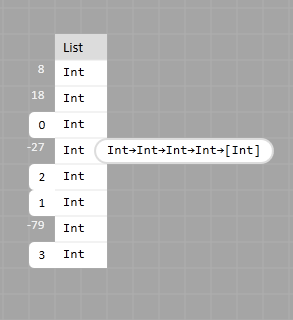
\includegraphics{img/partapply.PNG}
			\caption{Частично применённый конструктор списка}\label{part_list}
		\end{figure}
	Создать эффективный алгоритм, который бы переставил аргументы функции (конструктора) в нужном порядке, не представляется возможным. Поэтому для компонента, изображённого на рис.~\ref{part_list}, будет сгенерирован следующий код:
		
\begin{ListingEnv}[H]
	\begin{lstlisting}
root :: Int -> Int -> Int -> Int -> [Int]
root = \list1_arg0 list1_arg2 list1_arg1 list1_arg3 -> [8, 18, list1_arg0, -27, list1_arg2, list1_arg1, -79, list1_arg3]
	\end{lstlisting}
\end{ListingEnv}		

	
		Кратко рассмотрим генерацию кода функций. Для каждой функции необходимо сгенерировать её прототип (сигнатуру) и определение. Для сигнатуры нам понадобится конструктор \lstinline!SigD!, а для определения~--- \lstinline!FunD! (см. табл~\ref{decconstr}). Генерацией сигнатуры и определения будут заниматься соответственно функции 
		\begin{lstlisting}
generate_sig :: FunctionDef -> Dec
		\end{lstlisting}
		и
		\begin{lstlisting}
generate_body :: FunctionDef -> Dec.
		\end{lstlisting}		
		Каждая из них принимает выражение типа \lstinline!FunctionDef!, а возвращает выражение типа \lstinline!Dec!.		

		Наконец, все полученные выражения, которые сейчас имеют представление в виде типа данных \lstinline!Dec!, необходимо преобразовать к строке. Для этого определим функцию \lstinline!write_dec! с помощью стандартной функции \lstinline!ppr_dec! из фреймфорка Template Haskell (см. листинг~\ref{writedec}). Поскольку вторая возвращает выражение типа данных \lstinline!Doc!, для получения строки необходимо также применить метод \lstinline!show! класса типов \lstinline!Show!.

\begin{ListingEnv}[h]
	\begin{lstlisting}
write_dec :: Dec -> String
write_dec dec = (show $ ppr_dec False dec) ++ "\n"
	\end{lstlisting}
	\caption{Определение функции write\_dec}\label{writedec}
\end{ListingEnv}		

		Мы получили программу на языке Haskell, которая соответствует программе на визуальном языке программирования. Теперь определения из неё нужно передать в уже созданный GHC-контекст.

	\subsection{Компиляция кода и вычисление значения требуемой функции}\label{basefuns}
		В этом подразделе рассмотрим, каким образом новые определения добавляются в контекст. Кроме того, выясним, как затем вычислить нужное выражение.
		
		Благодаря функционалу GHC API добавить новые определение в уже созданный контекст не составляет труда. Воспользуемся функцией \lstinline!runDecls :: GhcMonad m => String -> m [Name]!. Она принимает строку, которая должна представлять из себя программу на языке Haskell, а возвращает список всех доступных пользователю имён (функций, конструкторов и т.д.). Определим функцию \lstinline!bringDeclsToCtxt! (см. листинг~\ref{bringDecls}). Она принимает контекст с уже имеющимися именами, программу на языке Haskell в виде строки и возвращает новый контекст, содержащий старые имена и те, что были в него помещены функцией \lstinline!runDecls!. В нашем случае эта функция может быть применена только к созданному выше контексту, в который помещены все возможные определения из различных модулей. Иначе программа на языке Haskell не сможет скомпилироваться.
		
		Также необходимо определить функцию, которая будет вычислять требуемое выражение и возвращать его значение. В нашем случае будет возвращаться строковое представление этого выражения. Итак, функция \lstinline!compileExps! (см. листинг~\ref{compileandrun}) принимает служебную строку (см. замечание~\ref{rem_force}), контекст и строку с выражением, которое нужно вычислить (см. замечание~\ref{rem_exp}). Возвращает эта функция результат внутри монады \lstinline!IO!. Здесь для вычисляемого выражения вызывается \lstinline!runExpression! (см. листинг~\ref{runexp}), в основе которой лежит функция библиотеки GHC API \lstinline!compileExpr!: она компилирует выражение, передаваемое ей в виде строки, и исполняет его.

\myremark{
	Служебная строка может принимать один из следующих видов:
	\begin{enumerate}[1)]
		\item \lstinline!"(return $ show ("!, если требуется вычислить выражение обычным образом;
		\item \lstinline|"(return $ show $!! ("|, если требуется вычислить выражение в "non-lazy" режиме (не лениво).
	\end{enumerate}
}\label{rem_force}

\myremark{
	Выражение для вычисления~--- обычное выражение, сконструированное с соблюдением синтаксиса языка Haskell, которое возвращает какое-либо значение. Например, <<\lstinline!3 + 3!>>, <<\lstinline|map (+ 3) [1, 2, 3]|>> и т.д. 
}\label{rem_exp}

\begin{ListingEnv}[h]
	\begin{lstlisting}
bringDeclsToCtxt :: Ghc [Name] -> String -> Ghc [Name]
bringDeclsToCtxt ctxt adts = ctxt >> (runDecls $ stringToDecls adts)
	\end{lstlisting}
	\caption{Определение функции bringDeclsToCtxt}\label{bringDecls}
\end{ListingEnv}		

\begin{ListingEnv}[h]
	\begin{lstlisting}
compileExp :: String -> Ghc a -> String -> IO b
compileExp mode ctxt xs = defaultErrorHandler defaultFatalMessager defaultFlushOut $
runGhc (Just libdir) $ (>>) ctxt $ (>>) runExpression
$ mode ++ x ++ ")) :: IO String") xs
	\end{lstlisting}
	\caption{Определение функции compileExp}\label{compileandrun}
\end{ListingEnv}

\begin{ListingEnv}
	\begin{lstlisting}
runExpression :: String -> Ghc b
runExpression exp = do
    act <- unsafeCoerce <$> compileExpr exp
    liftIO act
	\end{lstlisting}
	\caption{Определение функции runExpression}\label{runexp}
\end{ListingEnv}
	
	\subsection{Обработка исключений}
	На различных этапах работы транслятора могут возникать исключения. Здесь мы рассмотрим, как получить тексты сообщений этих исключений для дальнейшей отправки в основную программу.
	
	При создании контекста (\lstinline!createContext!) возможна ошибка отсутствия модуля с указанным именем (например, имя модуля было указано с опечаткой или же в текущей версии GHC этот модуль был упразднён). При добавлении новых определений в контекст (\lstinline!bringDeclsToCtxt!) возможны любые ошибки, которые только могут возникнуть при компиляции. То же самое справедливо и для функции \lstinline!compileExp!. Определим обёрточные функции \lstinline!tryCreateContext!, \lstinline!tryBringDeclsToCtxt! и \lstinline!tryCompileExp! (см. листинг~\ref{try}). Эти функции принимают те же аргументы, что и функции, которые они оборачивают, а возвращают выражение типа \lstinline!Either SomeException (Ghc [Name])!. Это значит, что если вычисления завершились успешно, результатом будет \lstinline!Right (Ghc [Name])!, в противном случае мы получим \lstinline!Left SomeException!. Каждая из этих функций вызывает \lstinline!tryEvaluate! (см. листинг~\ref{tryeval}) от результата оборачиваемой функции. При помощи стандартных функций библиотеки GHC API функция \lstinline!tryEvaluate! <<принудительно>> вычисляет выражение и получает исключение, если таковое возникло в результате его вычисления.

\begin{ListingEnv}[h]
	\begin{lstlisting}
tryCreateContext :: [String] -> IO (Either SomeException (Ghc [Name]))
tryCreateContext stdmods = tryEvaluate $ createContext stdmods

tryBringDeclsToCtxt :: Ghc [Name] -> String -> IO (Either SomeException (Ghc [Name]))
tryBringDeclsToCtxt ctxt adts = tryEvaluate $ bringDeclsToCtxt ctxt adts

tryCompileExp :: String -> Ghc a -> [String] -> IO (Either SomeException b)
tryCompileExp mode ctxt xs = (try :: IO a -> IO (Either SomeException a))
	$ compileExp mode ctxt xs
	\end{lstlisting}
	\caption{Определение функций tryCreateContext tryBringDeclsToCtxt, и tryCompileExp}\label{try}
\end{ListingEnv}	

\begin{ListingEnv}[h]
	\begin{lstlisting}
tryEvaluate = (try :: IO a -> IO (Either SomeException a)) . evaluate
	\end{lstlisting}
	\caption{Определение функции tryEvaluate}\label{tryeval}
\end{ListingEnv}
	
	Таким образом, если в процессе работы транслятора возникла ошибка, это не вызовет ошибки времени выполнения в основной программе. Кроме того, можно будет понять причину аварийного завершения программы на визуальном языке.
	
	\subsection{Взаимодействие между кодами на языках C++ и Haskell}	
	Наконец, необходимо предоставить возможность для основной программы (написанной на языке C++) вызвать функции, которые мы определили выше. Для этого воспользуемся средствами Foreign Function Interface. Для каждой из функций, описанных в подразделах~\ref{context} и~\ref{basefuns} определим специальным образом ещё несколько обёрточных функций. Согласно синтаксису Foreign Function Interface, для этих функций необходимо предварительно указать соглашение о вызове, которое будет для них использоваться (в данном случае соглашение о вызове языка C) (см. листинг~\ref{ccall}). В этих функциях использованы типы данных, уже пригодные для работы в языках C/C++. Поэтому их реализация будет заключаться в следующем:
	\begin{enumerate}[1)]
		\item преобразовать аргументы к типам данных языка Haskell;
		\item вызвать соответствующую функцию языка Haskell;
		\item преобразовать результат вызванной функции к типам данных для языка C/C++.
	\end{enumerate}

	Реализацию этих функций приводить не будем.

\begin{ListingEnv}
	\begin{lstlisting}
foreign export ccall c_create_context :: CWString -> IO (StablePtr (Either SomeException (Ghc [Name])))
foreign export ccall c_bring_decls_to_context :: StablePtr (Either SomeException (Ghc [Name])) 
              -> CWString 
              -> IO (StablePtr (Either SomeException (Ghc [Name])))
foreign export ccall c_compile_exps :: StablePtr (Either SomeException (Ghc a)) 
              -> CWString 
              -> IO (StablePtr (Either SomeException String))
	\end{lstlisting}
	\caption{FFI-заголовки функций c\_create\_context, c\_bring\_decls\_to\_context и c\_compile\_exps}\label{ccall}
\end{ListingEnv}	
	
\section{Пример работы транслятора}\label{transexample}
В этом разделе мы продемонстрируем, как работает реализованная нами программа, а также увидим в действии визуальный язык программирования.

Для демонстрации работы транслятора поступим следующим образом. Изобразим в IDE визуального языка программу. Для неё вручную напишем соответствующий ей код на языке Haskell, чтобы затем сравнить его с кодом, который даст транслятор. После скомпилируем и выполним обе программы и сравним результаты.

Изобразим программу вычисления длины целочисленного списка рекурсивным образом (см. рис. \ref{lengthrec}). 
\begin{figure}[p]
	\centering
	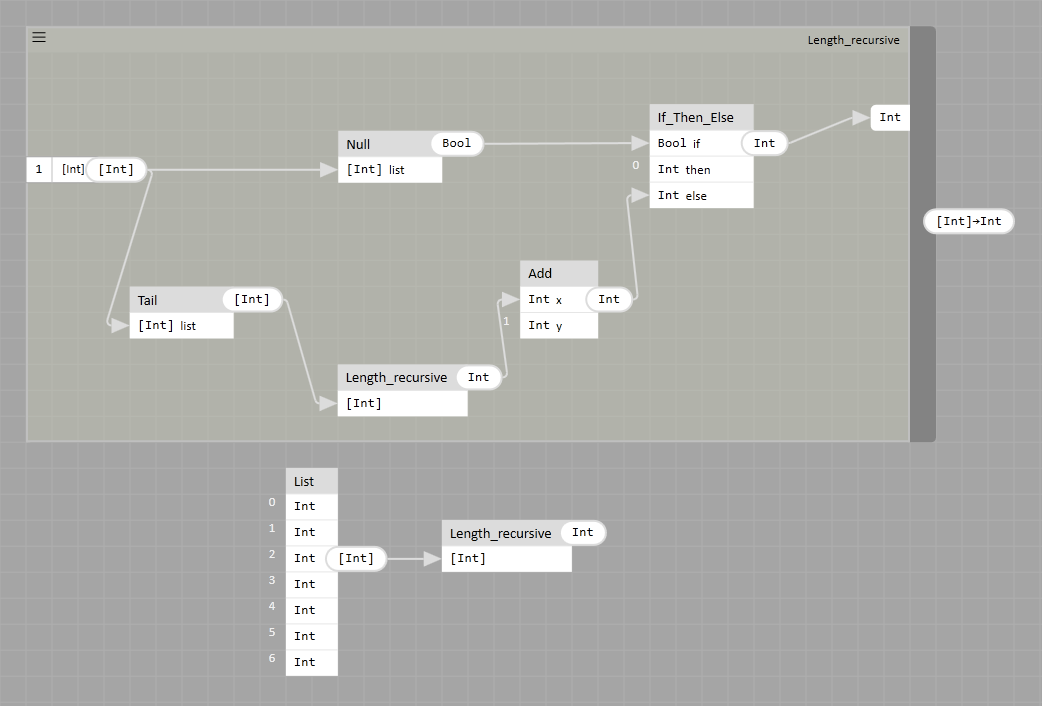
\includegraphics[width=\textwidth]{img/length.PNG}
	\caption{Реализация функции, вычисляющей длину списка, и её применение} \label{lengthrec}	
\end{figure}
Затем напишем код, который соответствует изображённому нами синтаксическому дереву (см. табл. \ref{expectreal}, левая колонка). 

Теперь получим промежуточное представление синтаксического дерева (см. листинг \ref{intermed}). Из промежуточного представления видно, что имеется две функции: основная функция, вычисляющая длину конкретного списка с помощью функции, определённой пользователем, и собственно функция вычисления длины списка, определённая пользователем. Основная функция не имеет аргументов и вложенных функций. Функция вычисления длины целочисленного списка имеет один аргумент (собственно список) и также не имеет вложенных функций. Это полностью отвечает тому, что мы изобразили в IDE.

Получаем код, который создаёт транслятор (см. табл. \ref{expectreal}, правая колонка). Видно, что он абсолютно идентичен коду, который был написан вручную: различаются только имена функций и их аргументов, порядок функций в программе.

Наконец, исполним функции с названием \lstinline!root! из обеих колонок табл. \ref{expectreal} и сравним результаты их вычислений. Результаты вычислений представлены в таблице \ref{exprealres}. Вычисление обеих функций дало одинаковый результат.


\begin{ListingEnv}[h]
\begin{lstlisting}
FunctionDef {
    fun_name = "root"
  , args = []
  , result = HsInt
  , body = Call (Custom "function1") (HsInt) 
          [Call (BuiltIn "list") (HsList (HsInt)) 
          [Literal HsInt "0"
         , Literal HsInt "1"
         , Literal HsInt "2"
         , Literal HsInt "3"
         , Literal HsInt "4"
         , Literal HsInt "5"
         , Literal HsInt "6"]]
  , nested_funs = []
 }
 
FunctionDef {
    fun_name = "function1"
  , args = [FunctionArg {
              arg_name = "function1_arg0"
            , arg_type = HsList (HsInt)}]
  , result = HsInt
  , body = Call (BuiltIn "if") (HsInt) 
          [Call (BuiltIn "null") (HsBool) 
          [Param "function1_arg0"]
        , Literal HsInt "0"
        , Call (Binary Add) (HsInt) 
          [Call (Custom "function1") (HsInt) 
          [Call (BuiltIn "tail") (HsList (HsInt)) 
          [Param "function1_arg0"]]
        , Literal HsInt "1"]]
  , nested_funs = []
 }
\end{lstlisting}
\caption{Промежуточное представление программы}\label{intermed}
\end{ListingEnv}

\begin{table}[h]
\centering
\begin{tabular}{|l|l|}
\hline
Код, написанный программистом &
Сгенерированный код \\
\hline
\begin{lstlisting}
length_rec :: [Int] -> Int
length_rec xs = 
 if null xs
  then 0
  else length_rec (tail xs) + 1

root :: Int
root = 
 length_rec [0, 1, 2, 3, 4, 5, 6]
\end{lstlisting} &
\begin{lstlisting}
root :: Int
root = 
 function1 [0, 1, 2, 3, 4, 5, 6]

function1 :: [Int] -> Int
function1 function1_arg0 = 
 if null function1_arg0
  then 0
  else 
   function1 (tail function1_arg0)
     + 1
\end{lstlisting} \\
\hline
\end{tabular}
\caption{Сравнение ожидаемого и сгенерированного кода}\label{expectreal}
\end{table}

\begin{table}[h]
\centering
\begin{tabular}{|l|l|}
\hline
Ожидаемые результаты & Полученные результаты \\
\hline
 & \\
\begin{minipage}{2in}
	\begin{verbatim}
*Main> root
7
	\end{verbatim}
\end{minipage} &
~~~~~~~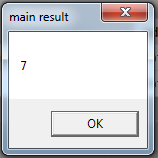
\includegraphics{img/result.PNG} \\
 & \\
\hline
\end{tabular}
\caption{Сравнение результатов вычислений ожидаемой и сгенерированной функции}\label{exprealres}
\end{table}

%\chapter{Тестирование}
%\section{Тест <<Переприсоединение>>}
%Тест <<Переприсоединение>> (англ. \textit{test-reconnect}) был задуман с целью автоматизации проверки того, что состояние контекста каждого компонента остаётся прежним после удаления и восстановления одной из входящих связей.
%\section{Тест <<Все ко всем>>}
%Тест <<Все ко всем>> (англ. \textit{all-to-all test}) воспроизводит попытки создания всевозможных явных связей (включая некорректные) для каждого конкретного примера. Это необходимо для проверки того, что все ошибочные ситуации обрабатываются правильно. К ошибочным ситуациям относятся:
%\begin{itemize}
%	\item попытка создания связи, которая приводит к циклу в синтаксическом дереве;
%	\item попытка создания связи, которая приводит к появлению бесконечного типа;
%\end{itemize}

\Conc
В ходе совместной с другими разработчиками языка работы над задачей был продуман и реализован алгоритм вывода типов для визуального языка в пределах одного компонента, алгоритм порядка обновления компонентов, а также решение было проверено на работоспособность в сравнении с языком-эталоном (Haskell). Помимо примера, рассмотренного в главе~\ref{transexample}, было разработано большое количество других тестовых примеров, на которых аналогичным образом была проверена работоспособность разработанного алгоритма. 

В результате работы мы приблизились к созданию первого тьюринг-полного функционального языка программирования с визуальным синтаксисом. Преимуществами данного языка программирования видятся наглядность и понятность работы системы типов и появление возможности наглядным образом изучить парадигму функционального программирования для тех, кто с ней не знаком. Кроме того, некоторые результаты будут использованы для развития основного разрабатываемого здесь программного продукта~--- Filter Forge.

% Печать списка литературы (библиографии)
\nocite{*}
\printbibliography[%{}
    heading=bibintoc%
    %,title=Библиография % если хочется это слово
]
% Файл со списком литературы: biblio.bib
% Подробно по оформлению библиографии:
% см. документацию к пакету biblatex-gost
% http://ctan.mirrorcatalogs.com/macros/latex/exptl/biblatex-contrib/biblatex-gost/doc/biblatex-gost.pdf
% и огромное количество примеров там же:
% http://mirror.macomnet.net/pub/CTAN/macros/latex/contrib/biblatex-contrib/biblatex-gost/doc/biblatex-gost-examples.pdf

%\appendix
%\ifthenelse{\value{worktype} > 1}{%
  %\addtocontents{toc}{%
      %\protect\renewcommand{\protect\cftchappresnum}{\appendixname\space}%
      %\protect\addtolength{\protect\cftchapnumwidth}{\widthof{\appendixname\space{}} - \widthof{Глава }}%
  %}%
%}{
  %\addtocontents{toc}{%
      %\protect\renewcommand{\protect\cftsecpresnum}{\appendixname\space}%
      %\protect\addtolength{\protect\cftsecnumwidth}{\widthof{\appendixname\space{}}}%
  %}%
%}

%\section{Пример работы программы}

%Здесь длинный листинг с примером работы.

\end{document}
